\documentclass[a4paper,10pt]{article}

\usepackage{amsmath,amssymb}
\usepackage{array}
\usepackage{booktabs}
\usepackage{geometry}
\usepackage{graphicx}
\usepackage{longtable}
\usepackage{tabularx}
\usepackage{tikz}
\usepackage{xurl}
\usetikzlibrary{arrows.meta,positioning,fit,calc,backgrounds}

\geometry{margin=18mm}
\pagestyle{plain}
\setlength{\parindent}{0pt}
\setlength{\parskip}{0.6em}
\sloppy
\urlstyle{tt}

\title{TALE-SD Waveform Graph Neural Network\\
Physics and Model Specification}
\author{}
\date{}

\newcommand{\code}[1]{\ifmmode\text{\ttfamily #1}\else\texttt{#1}\fi}
\newcommand{\pathcode}[1]{\begingroup\footnotesize\url{#1}\endgroup}
\newcolumntype{Y}{>{\raggedright\arraybackslash}X}
\newcommand{\R}{\mathbb{R}}

\begin{document}
\maketitle
\vspace{-7mm}

\section{Scope}

This document summarizes the physics-facing part of the TALE-SD waveform graph neural network.
It intentionally omits server paths, Slurm settings, run names, and other environment-dependent details.
The goal is to describe what enters the model, what the model predicts, and how the training losses are defined.

The current baseline is a joint reconstruction and mass-classification model.
It reconstructs the shower energy, core position, and arrival direction, predicts a reconstruction-quality score, and can classify the primary particle as proton or iron.

\section{Implementation Map}

This section maps the model description to the source code.
The production workflow has two distinct stages: exporting DST events into HDF5 graphs, and training from those HDF5 graphs.
The overall data flow is
\begin{footnotesize}
\[
\begin{aligned}
\mathrm{DST}
&\rightarrow
\code{talesd-gnn export}
\rightarrow
\mathrm{HDF5\ graph}
\rightarrow
\code{H5GraphDataset}
\\
&\rightarrow
\code{train\_model}
\rightarrow
\code{PhysicsTaleSdGNN}
\rightarrow
\mathrm{loss/metrics/diagnostics}.
\end{aligned}
\]
\end{footnotesize}

\begin{table}[htbp]
  \centering
  \caption{Main implementation stages and source files.}
  \label{tab:en-implementation-map}
  {\footnotesize
  \begin{tabularx}{\linewidth}{>{\raggedright\arraybackslash}p{27mm}Y Y}
    \toprule
    Stage & Main file & Role \\
    \midrule
    CLI entry point &
    \pathcode{src/talesd_gnn_reconstruction/cli.py} &
    Parses \code{talesd-gnn} subcommands and maps command-line options to Python API arguments. \\
    DST reading &
    \pathcode{src/talesd_gnn_reconstruction/dst_reader.py} &
    Iterates DST banks and produces records for graph construction. \\
    Event graph creation &
    \pathcode{src/talesd_gnn_reconstruction/event_graph.py} &
    Builds accepted-pulse nodes, edges, waveforms, targets, and metadata. \\
    HDF5 writing &
    \pathcode{src/talesd_gnn_reconstruction/graph_io.py} &
    Writes graph shards and stores schema attributes such as \code{columns\_json} and \code{waveform\_schema}. \\
    HDF5 loading &
    \pathcode{src/talesd_gnn_reconstruction/dataset.py} &
    Presents one file or many shards as a PyTorch-compatible dataset. \\
    Training workflow &
    \pathcode{src/talesd_gnn_reconstruction/train.py} &
    Handles split, scalers, DataLoaders, epoch loop, losses, best checkpoint, and final evaluation. \\
    Model &
    \pathcode{src/talesd_gnn_reconstruction/model.py} &
    Embeds node, edge, and waveform inputs, applies message passing and graph readout, and returns task heads. \\
    Diagnostics &
    \pathcode{src/talesd_gnn_reconstruction/diagnostics.py} &
    Writes learning curves, energy-dependence plots, quality-cut plots, and mass diagnostics. \\
    Feature analysis &
    \pathcode{src/talesd_gnn_reconstruction/feature_analysis.py} &
    Writes input distributions and post-hoc feature-group ablation results. \\
    \bottomrule
  \end{tabularx}
  }
\end{table}

The command-line interface is a thin wrapper.
For example, \code{cli.\_cmd\_train} calls \code{train.train\_model}; the heavy work is not implemented in the parser itself.
The central training function creates the dataset, constructs the train/validation/test split, fits scalers on the training split, builds DataLoaders, runs the epoch loop, saves the best validation checkpoint, and performs final validation/test evaluation.
The neural network class \code{PhysicsTaleSdGNN} only performs the forward pass.
Losses are computed in \code{train.py}, which keeps reconstruction, quality, mass, and bias-penalty terms separate from the model architecture.

\subsection{Heterogeneous graph workflow}

The implementation now also contains a heterogeneous graph path based on the public \code{dstio.tale.graph} API.
This path is separate from the accepted-pulse homogeneous HDF5 schema described in the following sections.
It represents detector readouts and pulse candidates as two node types rather than duplicating detector waveforms on every pulse node.
Detector waveforms are stored once on detector nodes, and pulse nodes refer to their detector through the detector--pulse relation and pulse bounds.
The graph relations are pulse--pulse, detector--detector, and detector--pulse relations.

\begin{figure}[tbp]
  \centering
  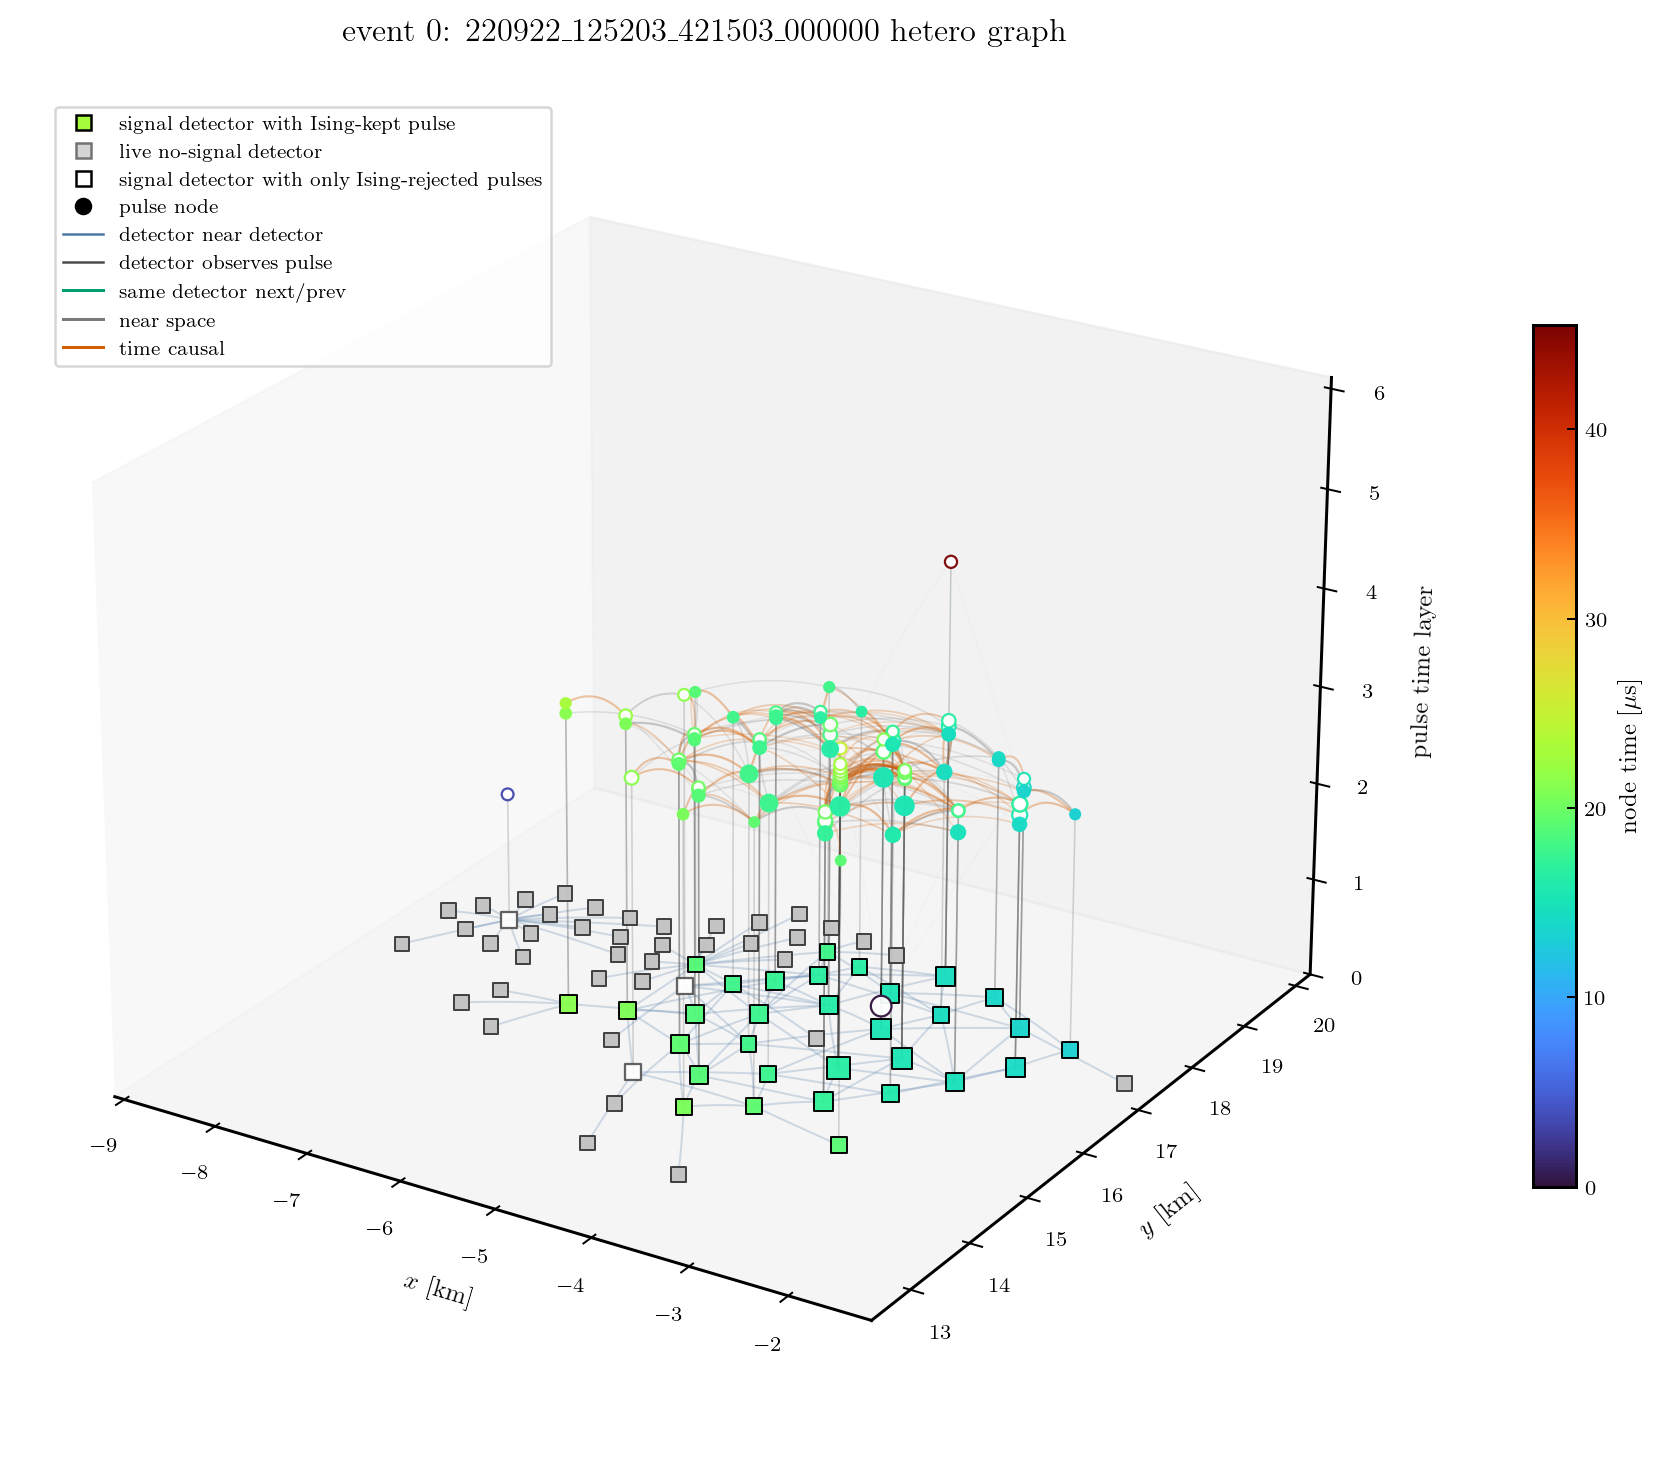
\includegraphics[width=0.95\linewidth]{fig/hetero_graph_event_display.png}
  \caption{
    Heterogeneous graph display for one real event.
    Square markers are detector nodes and round markers are pulse nodes.
    Filled detector squares have at least one Ising-kept pulse; gray squares are live no-signal detector nodes; open detector squares have only Ising-rejected pulse candidates.
    Pulse nodes are drawn above their detector on a pulse-time layer and are connected back to their detector by vertical detector--pulse edges.
    Blue edges are detector--detector proximity relations, green edges connect consecutive pulses on the same detector, gray pulse--pulse edges are near-space relations, and orange pulse--pulse edges are the time-causal subset.
  }
  \label{fig:hetero-graph-event-display}
\end{figure}

For comparison, Figure~\ref{fig:homogeneous-graph-event-display-kept-only}
shows the same event after removing detector nodes and rejected pulses from the
display.  This view matches the pulse nodes and pulse--pulse edges used when a
homogeneous comparison graph is made from the heterogeneous HDF5 with
\code{PULSE\_MASK=ising\_kept}.

\begin{figure}[tbp]
  \centering
  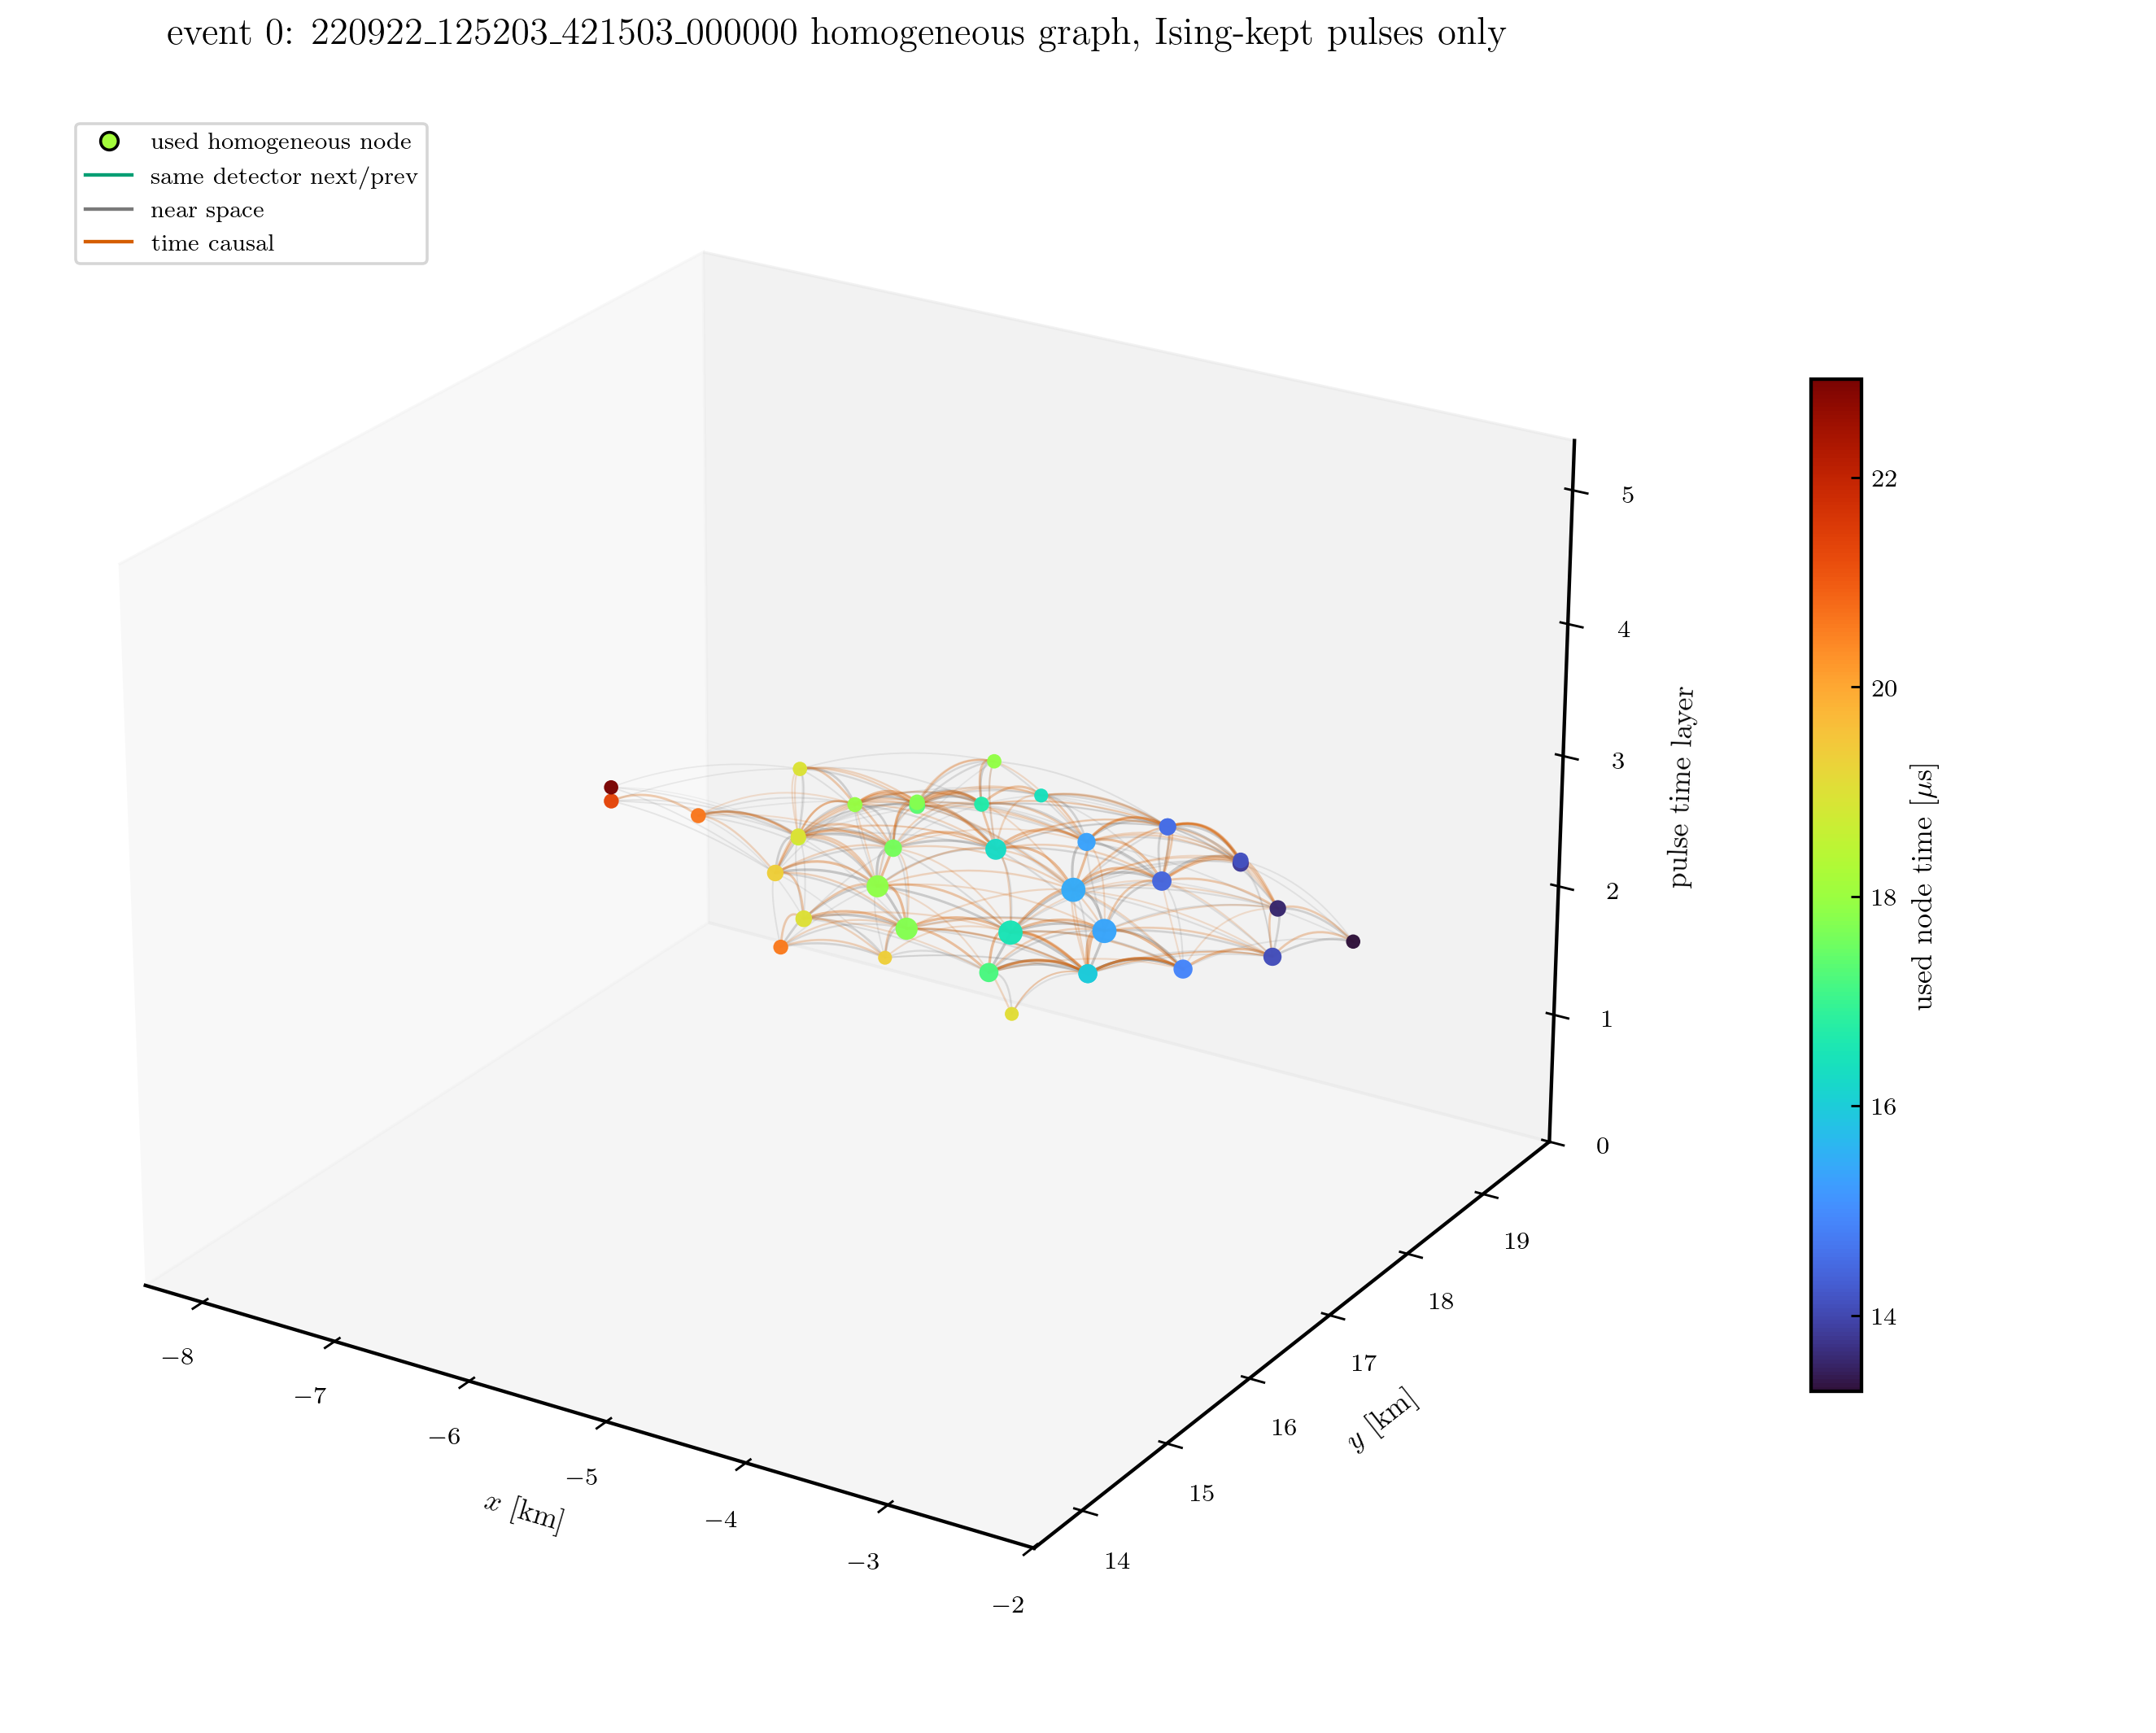
\includegraphics[width=0.95\linewidth]{fig/homogeneous_graph_event_display_ising_kept_only.png}
  \caption{
    Homogeneous pulse graph display with only Ising-kept pulses drawn.
    Detector nodes, detector edges, and Ising-rejected pulse nodes are not
    drawn.  Color encodes the time of the used pulse nodes, and edges are shown
    only between used pulses.
  }
  \label{fig:homogeneous-graph-event-display-kept-only}
\end{figure}

Figure~\ref{fig:hetero-graph-event-display} shows why the model input is not a single homogeneous node table.
Detector nodes carry detector-level features and detector waveforms, while pulse nodes carry pulse-candidate features and Ising annotations.
The model therefore encodes detector features, detector waveforms, pulse features, and typed edge relations as separate inputs before message passing.

The heterogeneous training/cache path is
\begin{footnotesize}
\[
\mathrm{DST}
\rightarrow
\code{talesd-gnn export-hetero}
\rightarrow
\mathrm{heterogeneous\ HDF5\ graph}
\rightarrow
\code{train-hetero}
\rightarrow
\code{MinimalHeteroTaleSdGNN}.
\]
\end{footnotesize}
The final one-pass reconstruction path does not require an intermediate HDF5 file:
\begin{footnotesize}
\[
\mathrm{DST}
\rightarrow
\code{talesd-gnn reconstruct-dst}
\rightarrow
\code{dstio.tale.graph.iter\_graphs}
\rightarrow
\code{MinimalHeteroTaleSdGNN}
\rightarrow
\mathrm{reconstruction\ CSV}.
\]
\end{footnotesize}
For this path, HDF5 is a training cache only.
The direct reconstruction command and the HDF5 exporter use the same graph schema, feature conversion layer, and checkpoint scalers.
The current comparison to run for this path is reco+mass with either the quality head enabled or the predicted-error head enabled, while keeping \code{LOSS\_MODE=physics}.

\section{Event Graph Input}

One air-shower event is represented as one directed graph.
The graph nodes are accepted coincidence pulses after the Ising-style noise filter.
If one detector has multiple accepted pulses, each pulse becomes a separate node.
Events with fewer than four pulse nodes or fewer than four distinct detectors are not used.

The HDF5 graph representation contains the tensors in Table~\ref{tab:tensors}.

\begin{table}[htbp]
  \centering
  \caption{Main tensors for one event graph.}
  \label{tab:tensors}
  \begin{tabular}{lll}
    \toprule
    Tensor & Shape & Meaning \\
    \midrule
    $\mathbf{X}$ & $N_v\times28$ & Accepted-pulse node scalar features. \\
    $\mathbf{A}$ & $N_e\times13$ & Directed-edge scalar features. \\
    $\mathbf{P}_{\mathrm{raw}}$ & $N_p\times1$ & Pulse-to-node index only. \\
    $\mathbf{W}$ & $N_v\times4\times128$ & Four waveform channels per pulse node. \\
    $\mathbf{y}_{\mathrm{reco}}$ & $6$ & Reconstruction target. \\
    $y_{\mathrm{mass}}$ & $1$ & Proton/iron label when MC truth is available. \\
    \bottomrule
  \end{tabular}
\end{table}

The 28 node scalar features are attached to accepted-pulse nodes.
The row unit is an accepted pulse, not a detector.
Each row nevertheless contains a controlled mixture of pulse-derived, detector-derived, and event-context quantities:
\begin{itemize}
  \item detector-derived quantities: detector position, local detector spacing, trigger time, pedestal, pedestal RMS, waveform length, waveform segment count, and FADC peak;
  \item pulse-derived quantities: the accepted pulse's own arrival time, signal density $\rho$, accepted-pulse order within the detector, and first-pulse flag;
  \item detector pulse-context quantities: accepted-pulse count, accepted-pulse time span, maximum accepted-pulse signal, and summed accepted-pulse signal in the same detector;
  \item event-context quantities: position relative to the signal-weighted event barycenter.
\end{itemize}
Thus $\mathbf{X}$ should be read as scalar features attached to accepted-pulse nodes, not as detector-node features.
The standard model does not use a learned detector-ID embedding.
Detector-dependent behavior is instead learned from coordinates, local spacing, calibration/noise quantities, waveforms, and graph connectivity.

The current $\mathbf{P}_{\mathrm{raw}}$ keeps only the node index that maps each accepted pulse back to its node.
Older HDF5 files stored six additional pulse-scalar columns, but they duplicate the accepted-pulse node features and are not used.
Because the node-feature semantics have been redefined, old HDF5 files are not silently migrated to the current 28-column schema; the graph files must be re-exported.

Each node also carries four calibrated waveform channels:
\[
\mathbf{W}_v =
\left(
W^u_{\mathrm{raw}},
W^l_{\mathrm{raw}},
M^u_{\mathrm{accepted}},
M^l_{\mathrm{accepted}}
\right)\in\R^{4\times128}.
\]
The raw channels are rise-aligned windows around the accepted pulse.
The mask channels use the same time axis as the raw windows and mark accepted-pulse intervals with 1 and all other bins with 0.
Thus waveform amplitudes and accepted-pulse selection are passed as separate inputs.
One bin corresponds to $0.02\,\mu\mathrm{s}$, so 128 bins cover $2.56\,\mu\mathrm{s}$.

Edges are drawn only between pulse nodes from different detectors.
An undirected detector pair is accepted if the distance is at most $1.5\,\mathrm{km}$ and the time difference satisfies $|\Delta t|\le8\,\mu\mathrm{s}$.
Each accepted pair is stored as two directed edges.
For edge $i\rightarrow j$, the edge features include
\[
(\Delta x,\Delta y,\Delta z,d,\Delta t,|\Delta t|,\Delta t/d,
\Delta\log_{10}\rho,
w_{\mathrm{ising}},w_{\mathrm{raw}},t_{\mathrm{excess}},s_{\mathrm{space}},s_{\mathrm{causal}}).
\]
Here
\[
  s_{\mathrm{space}}=\exp(-d/0.8\,\mathrm{km}),\qquad
  t_{\mathrm{excess}}=\max(0,|\Delta t|-d/c-0.3\,\mu\mathrm{s}),
\]
\[
  s_{\mathrm{causal}}=\exp(-t_{\mathrm{excess}}/1.0\,\mu\mathrm{s}),
\]
and
\[
  w_{\mathrm{raw}}
  =
  s_{\mathrm{space}}s_{\mathrm{causal}}
  \left[
    1+0.12\sqrt{\log(1+\rho_i)\log(1+\rho_j)}
  \right].
\]
The Ising-style weight is degree-normalized as
\[
  w_{\mathrm{ising}} =
  \frac{w_{\mathrm{raw}}}{(D_iD_j)^{0.35}},
\]
where $D_i$ and $D_j$ are positive connection counts.

\section{Input Distribution Diagnostics}

Figures~\ref{fig:en-input-node}, \ref{fig:en-input-edge}, and~\ref{fig:en-input-pulse-waveform-target} show input distributions generated from the current HDF5 export, \pathcode{flat50000_wfmask_target6_20260603_102418}.
This export contains 2,839,184 events in 29 shards: 1,455,815 proton events and 1,383,369 iron events.
The plots use a 100,000-event sample.
In the current schema, pulse-level quantities such as \code{log10\_pulse\_rho} are separated from detector-level accepted-pulse aggregates such as \code{log10\_detector\_sum\_pulse\_rho} and \code{detector\_accepted\_pulse\_count}.
The waveform channels are \code{upper\_raw\_window\_vem}, \code{lower\_raw\_window\_vem}, \code{upper\_accepted\_mask}, and \code{lower\_accepted\_mask}.
The current \code{pulse\_features} tensor keeps only \code{node\_index}, so no additional pulse-scalar distribution is shown.
Figure~\ref{fig:en-split-distributions} shows the train/validation/test distributions for the same HDF5 export.
The split is performed by source group rather than by raw event index.
Usually the source group is the raw source path.
For split CORSIKA DST files named like \code{DAT??????\_gea\_trg\_XXX.dst.gz}, all \code{XXX} chunks with the same \code{DAT??????} shower id must remain in the same split.
The existing summary for this export reports event fractions of 81.0\%, 7.37\%, and 11.6\%, and raw source-path fractions of 69.3\%, 10.1\%, and 20.6\%.
Those source counts were generated before the CORSIKA chunk grouping correction, so the source-group fractions must be regenerated from the HDF5 summary.
The event fractions can differ from the nominal target because the split preserves source-group separation.
These plots are input diagnostics, not trained-model performance metrics.
No event-level graph topology figure is included here because no current-analysis graph PDF has been generated from this HDF5 export.
Older graph PDFs from other checks or analyses are intentionally not used as figures for this model description.

\begin{figure}[p]
  \centering
  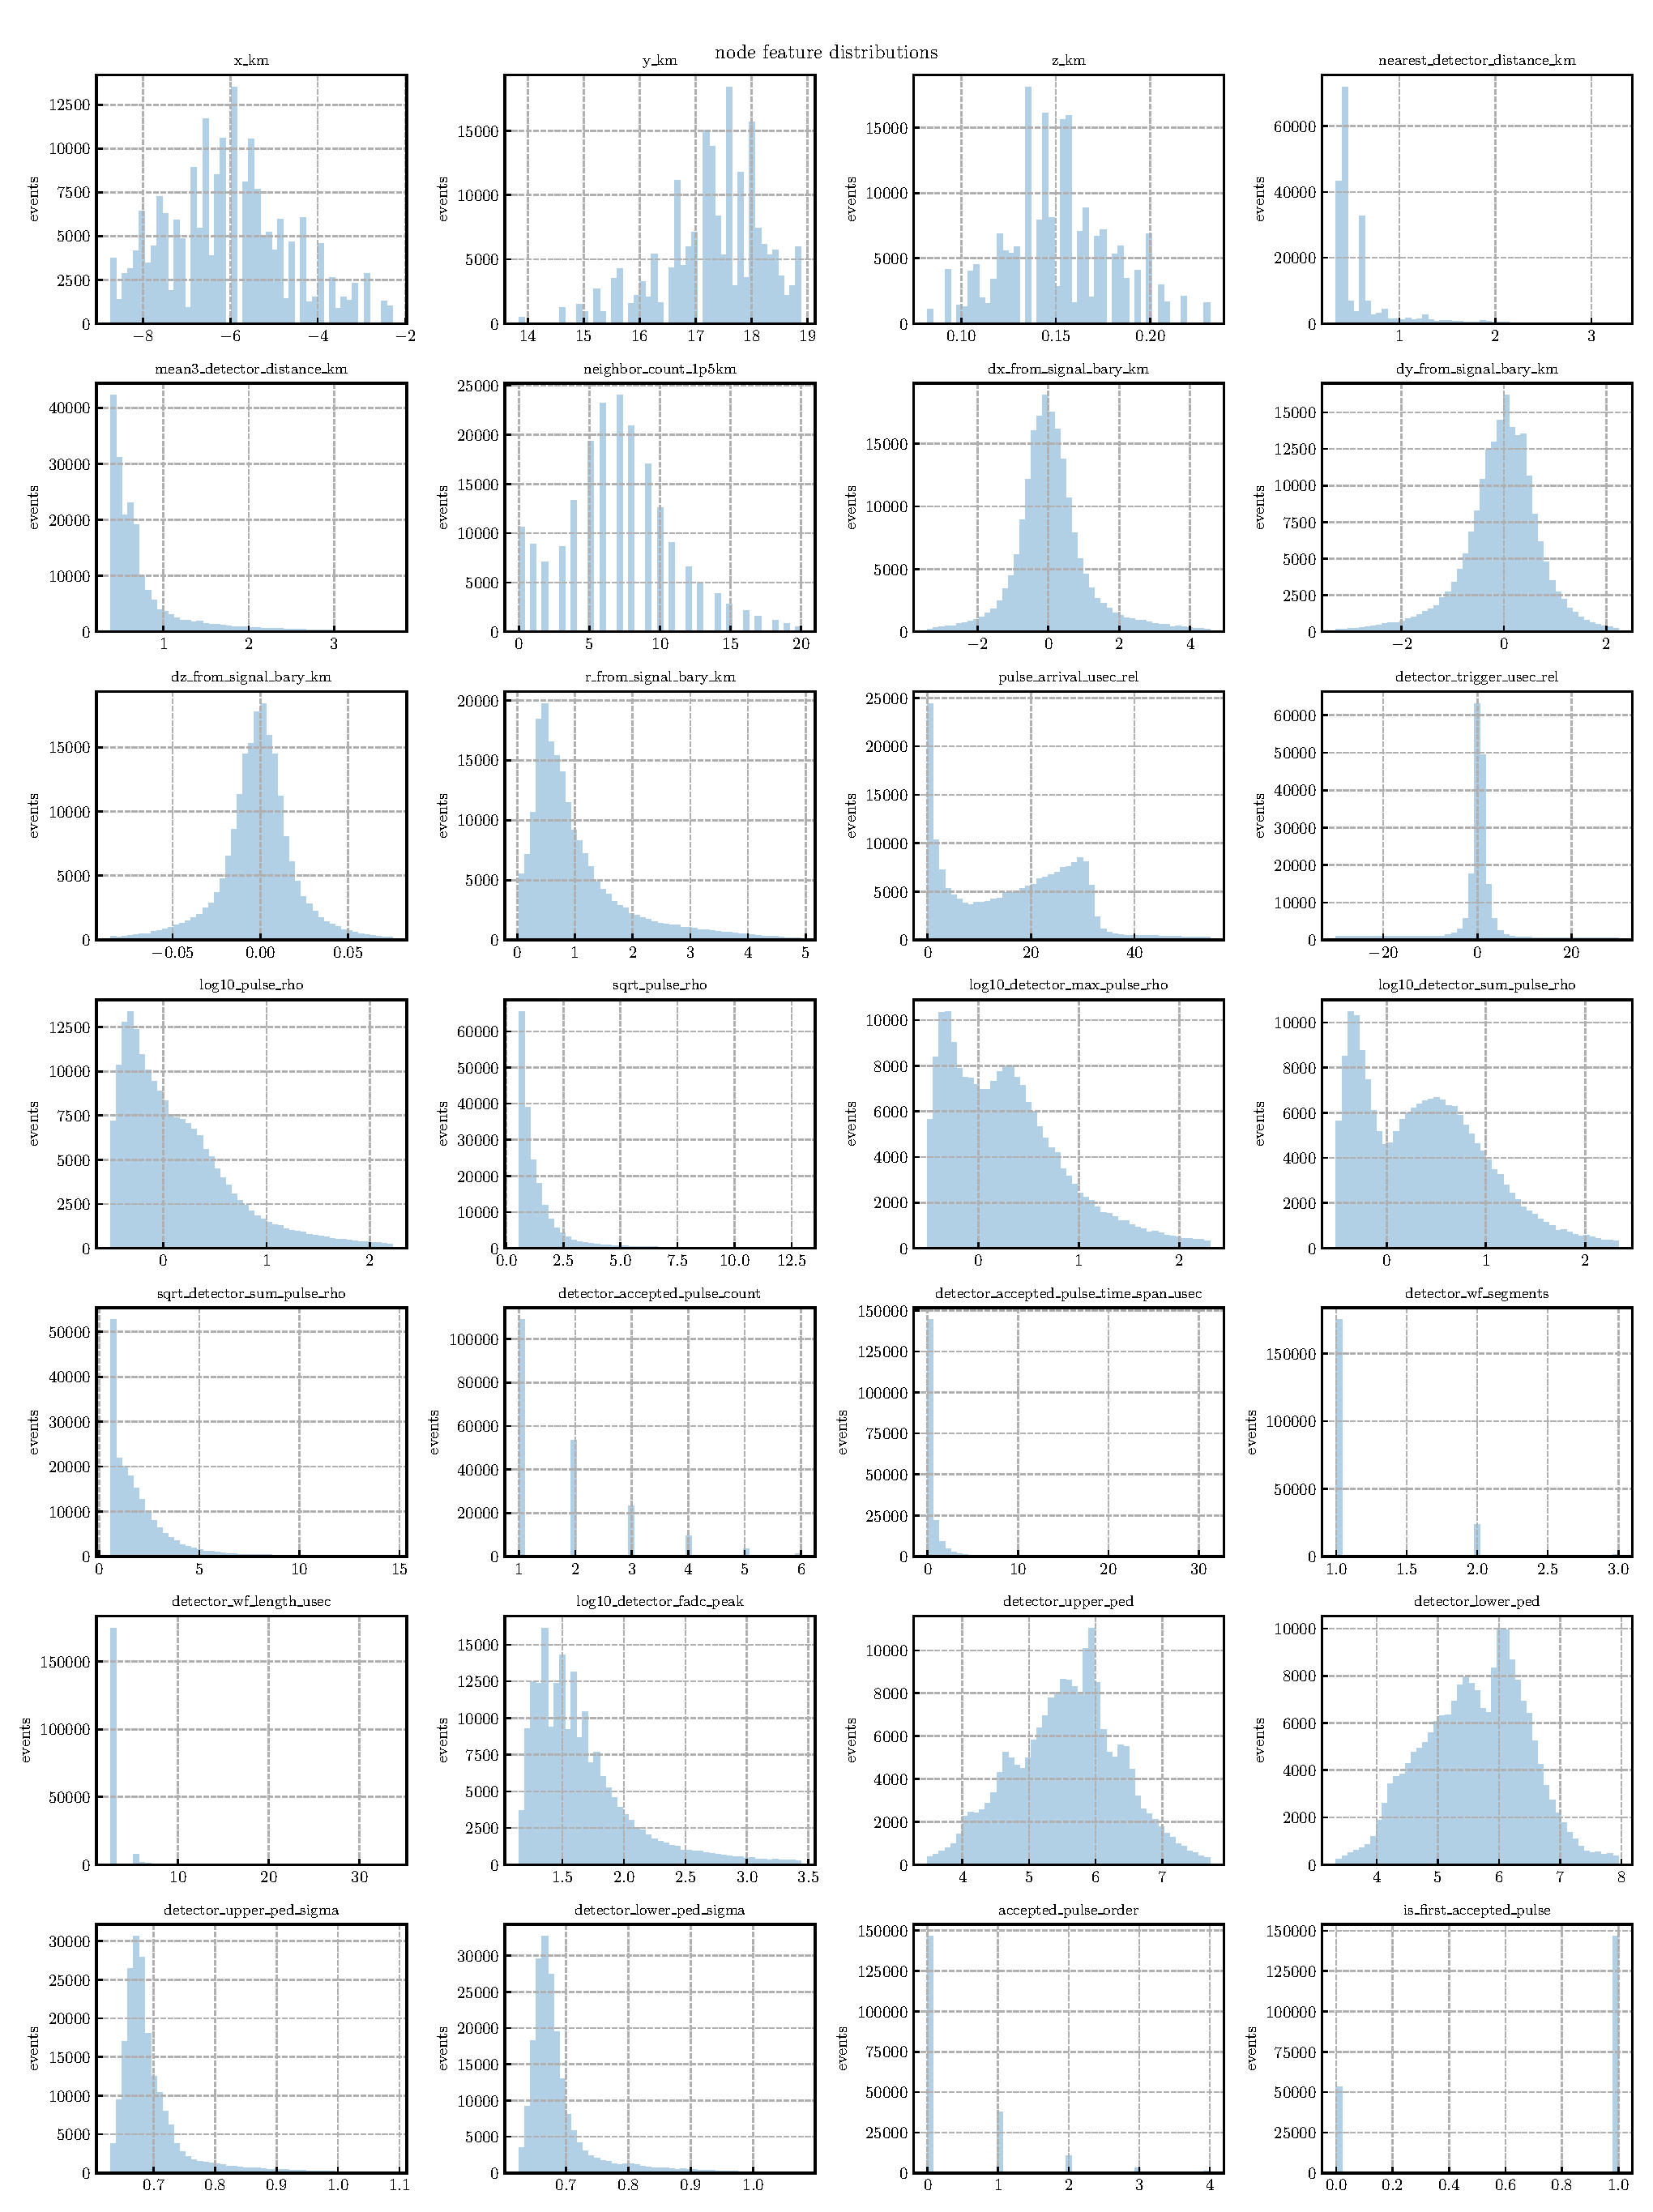
\includegraphics[width=0.95\linewidth]{fig/input_distributions/node_features.pdf}
  \caption{Accepted-pulse node-feature distributions from the current HDF5 export.}
  \label{fig:en-input-node}
\end{figure}

\begin{figure}[p]
  \centering
  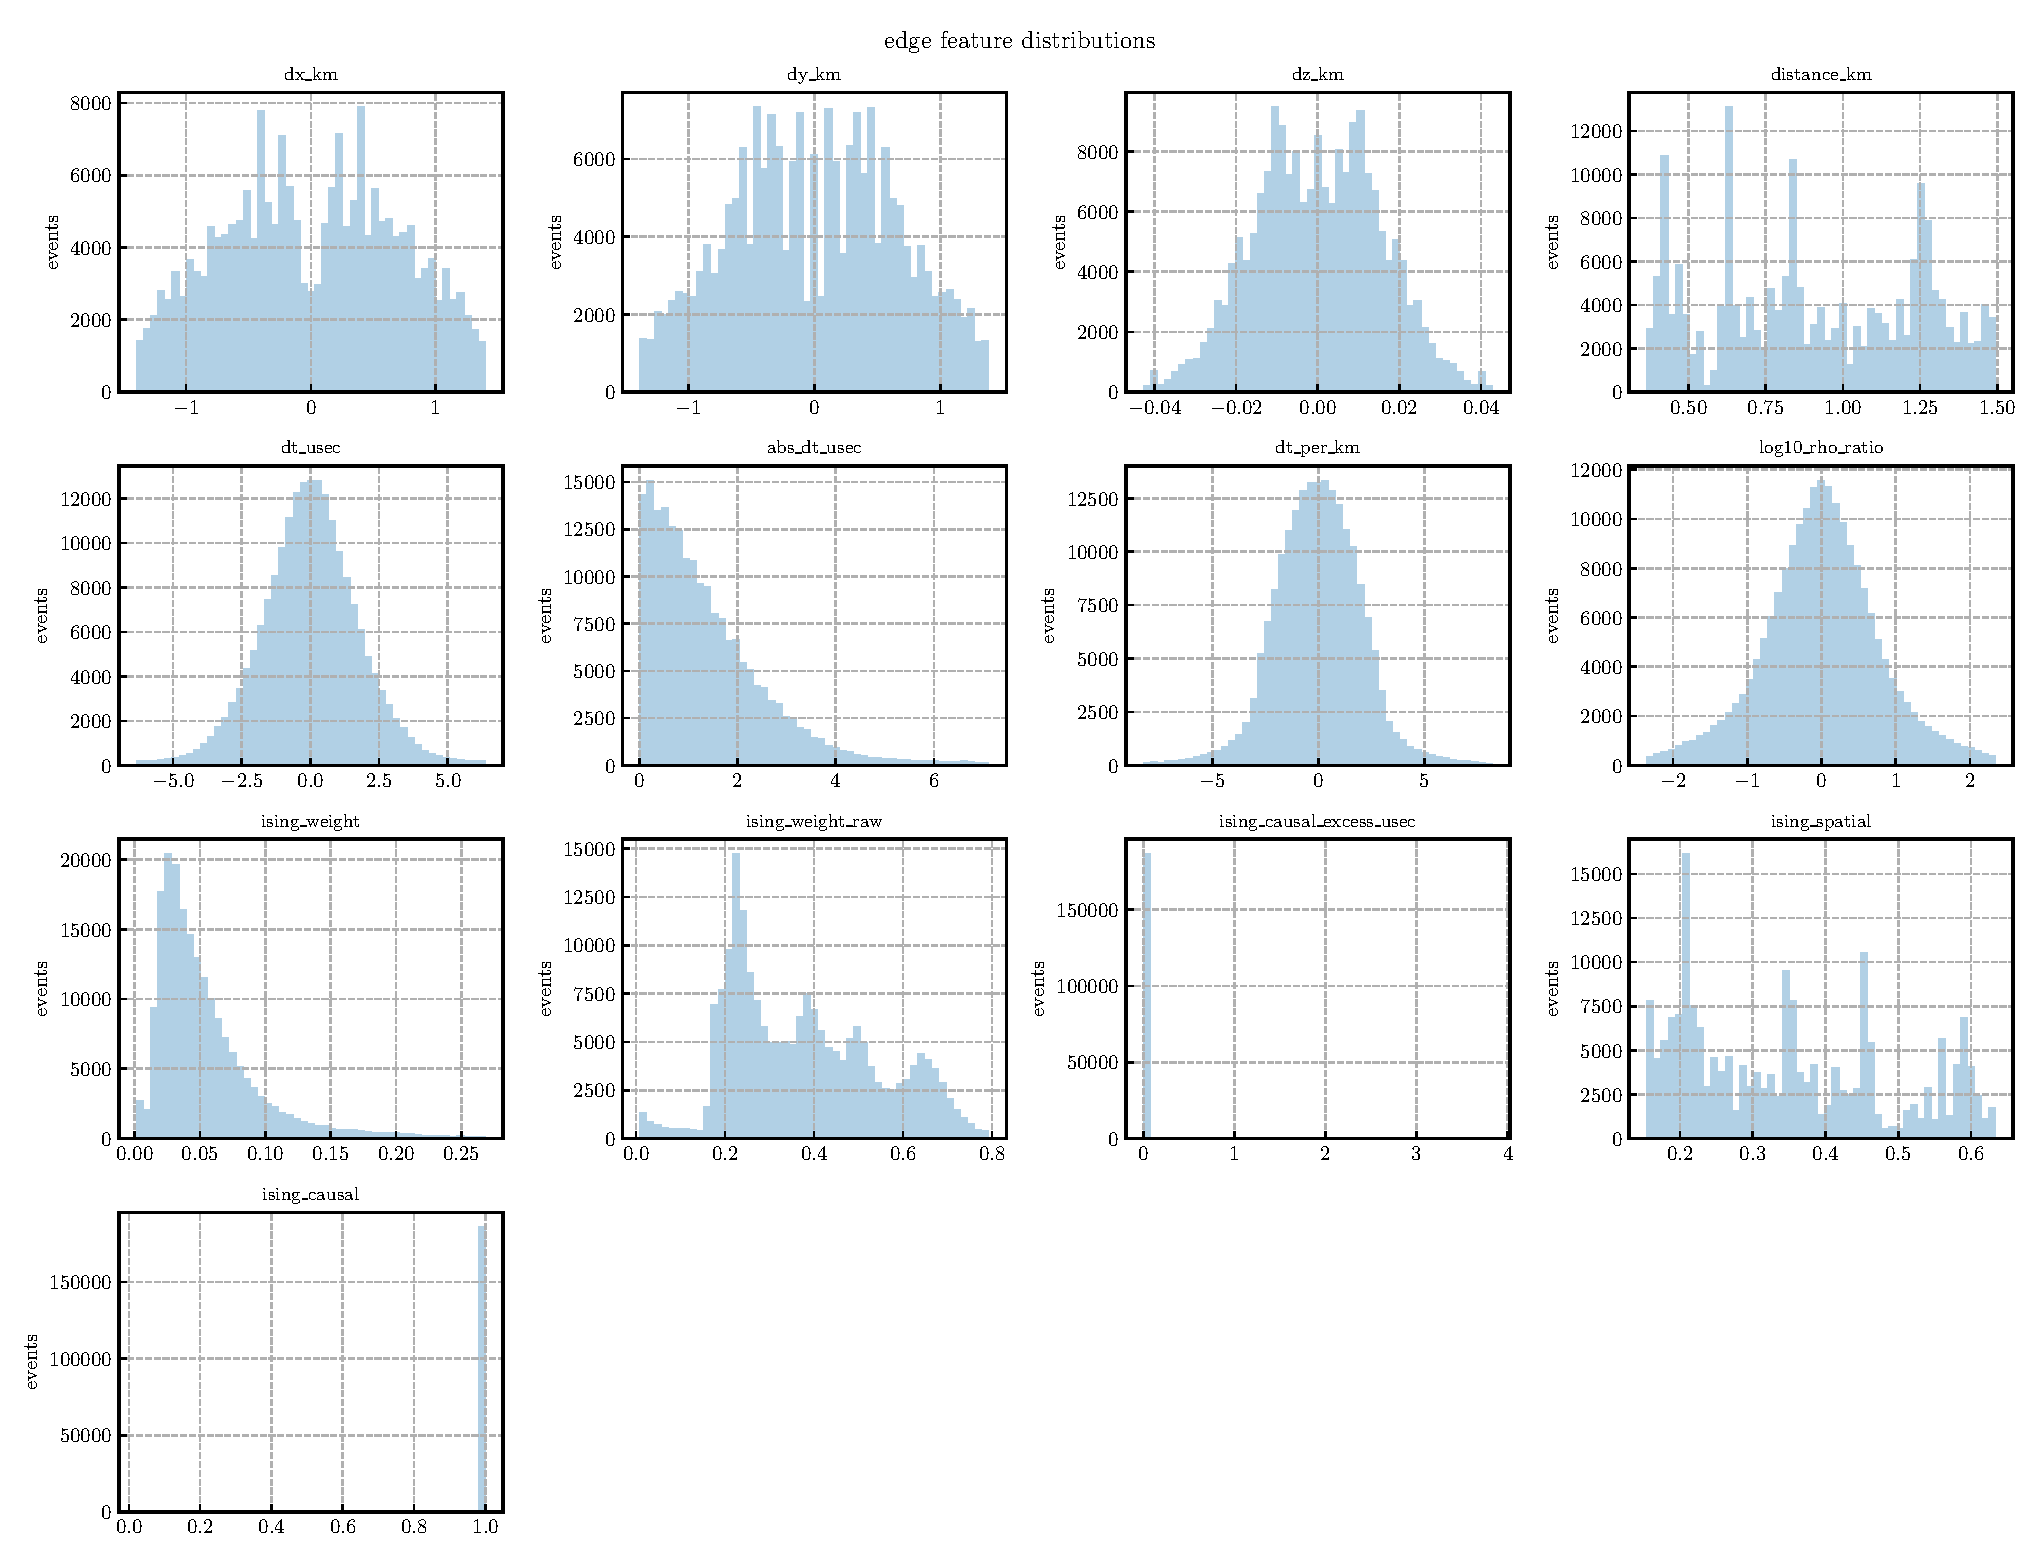
\includegraphics[width=0.95\linewidth]{fig/input_distributions/edge_features.pdf}
  \caption{Edge-feature distributions from the current HDF5 export.}
  \label{fig:en-input-edge}
\end{figure}

\begin{figure}[p]
  \centering
  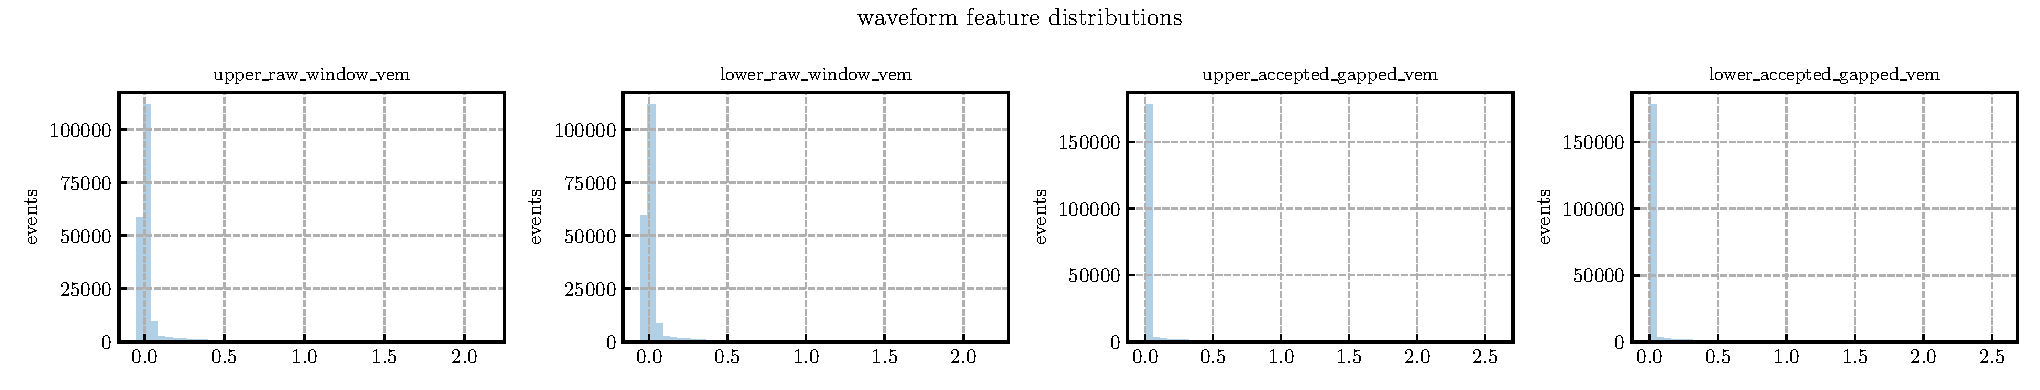
\includegraphics[width=0.95\linewidth]{fig/input_distributions/waveform_features.pdf}
  \vspace{2mm}
  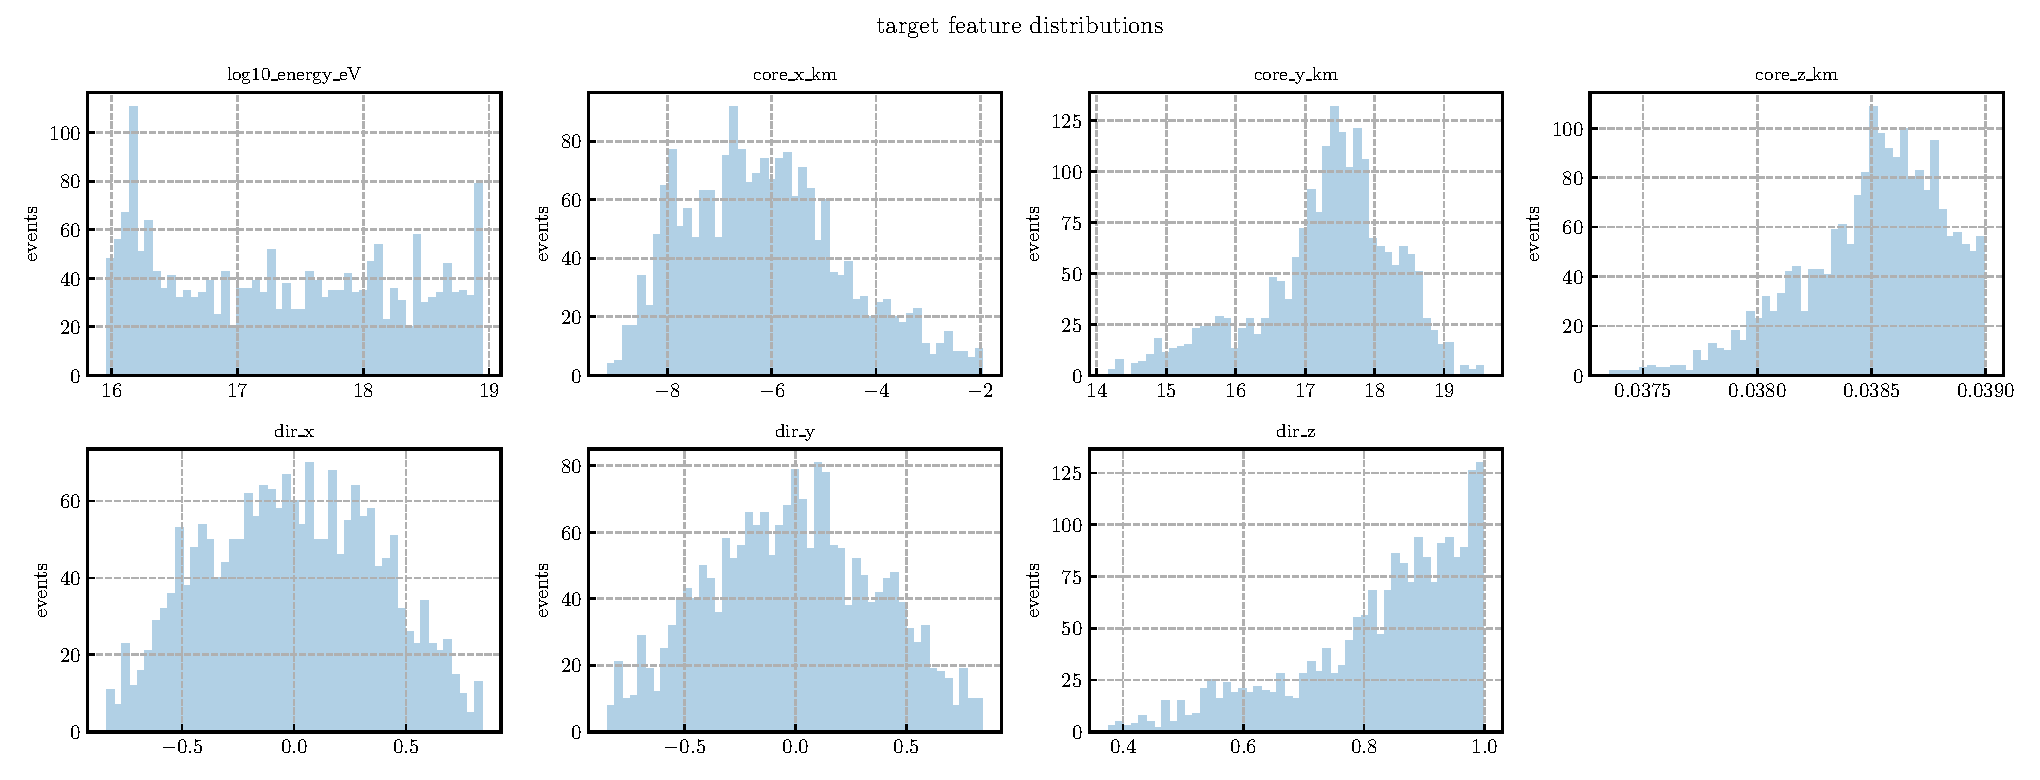
\includegraphics[width=0.95\linewidth]{fig/input_distributions/target_features.pdf}
  \caption{Waveform-feature and reconstruction-target distributions from the current HDF5 export.}
  \label{fig:en-input-pulse-waveform-target}
\end{figure}

\begin{figure}[p]
  \centering
  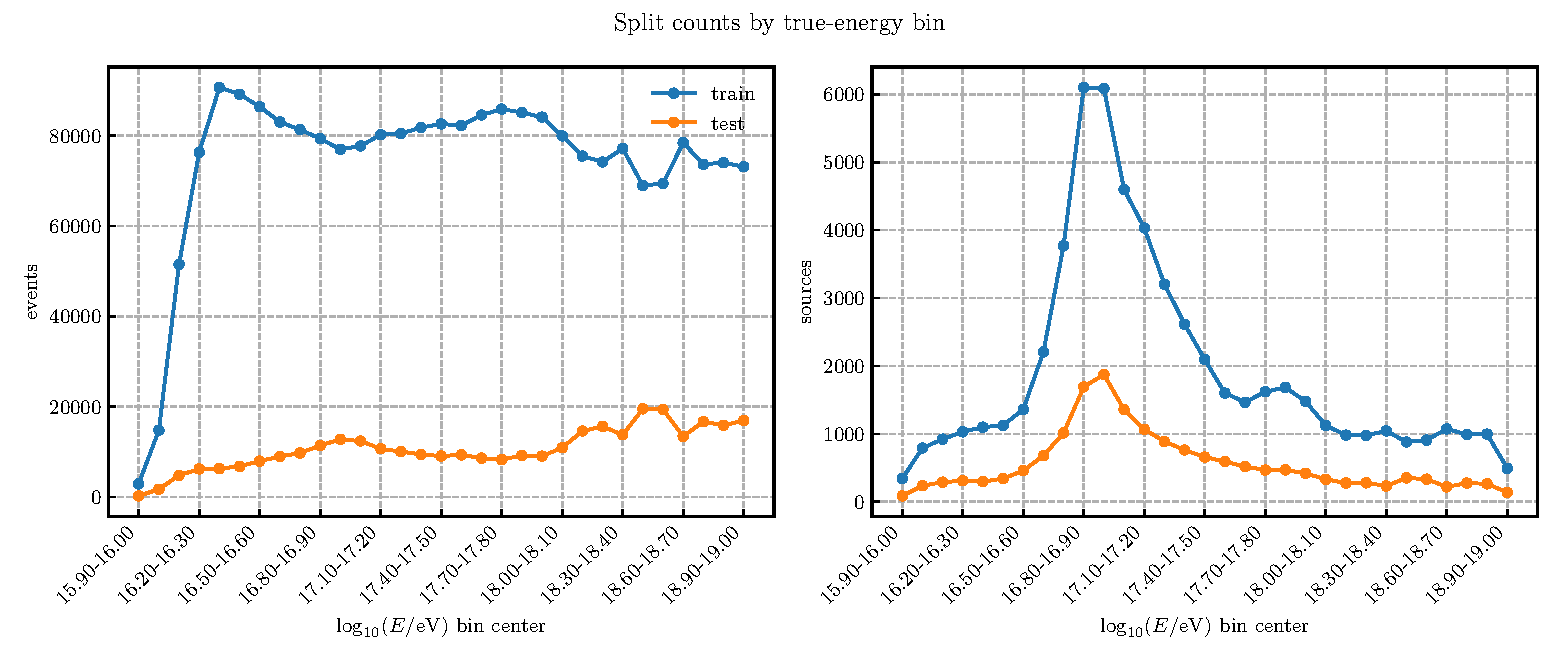
\includegraphics[width=0.95\linewidth]{fig/split_distributions/split_energy_bin_counts.pdf}
  \vspace{2mm}
  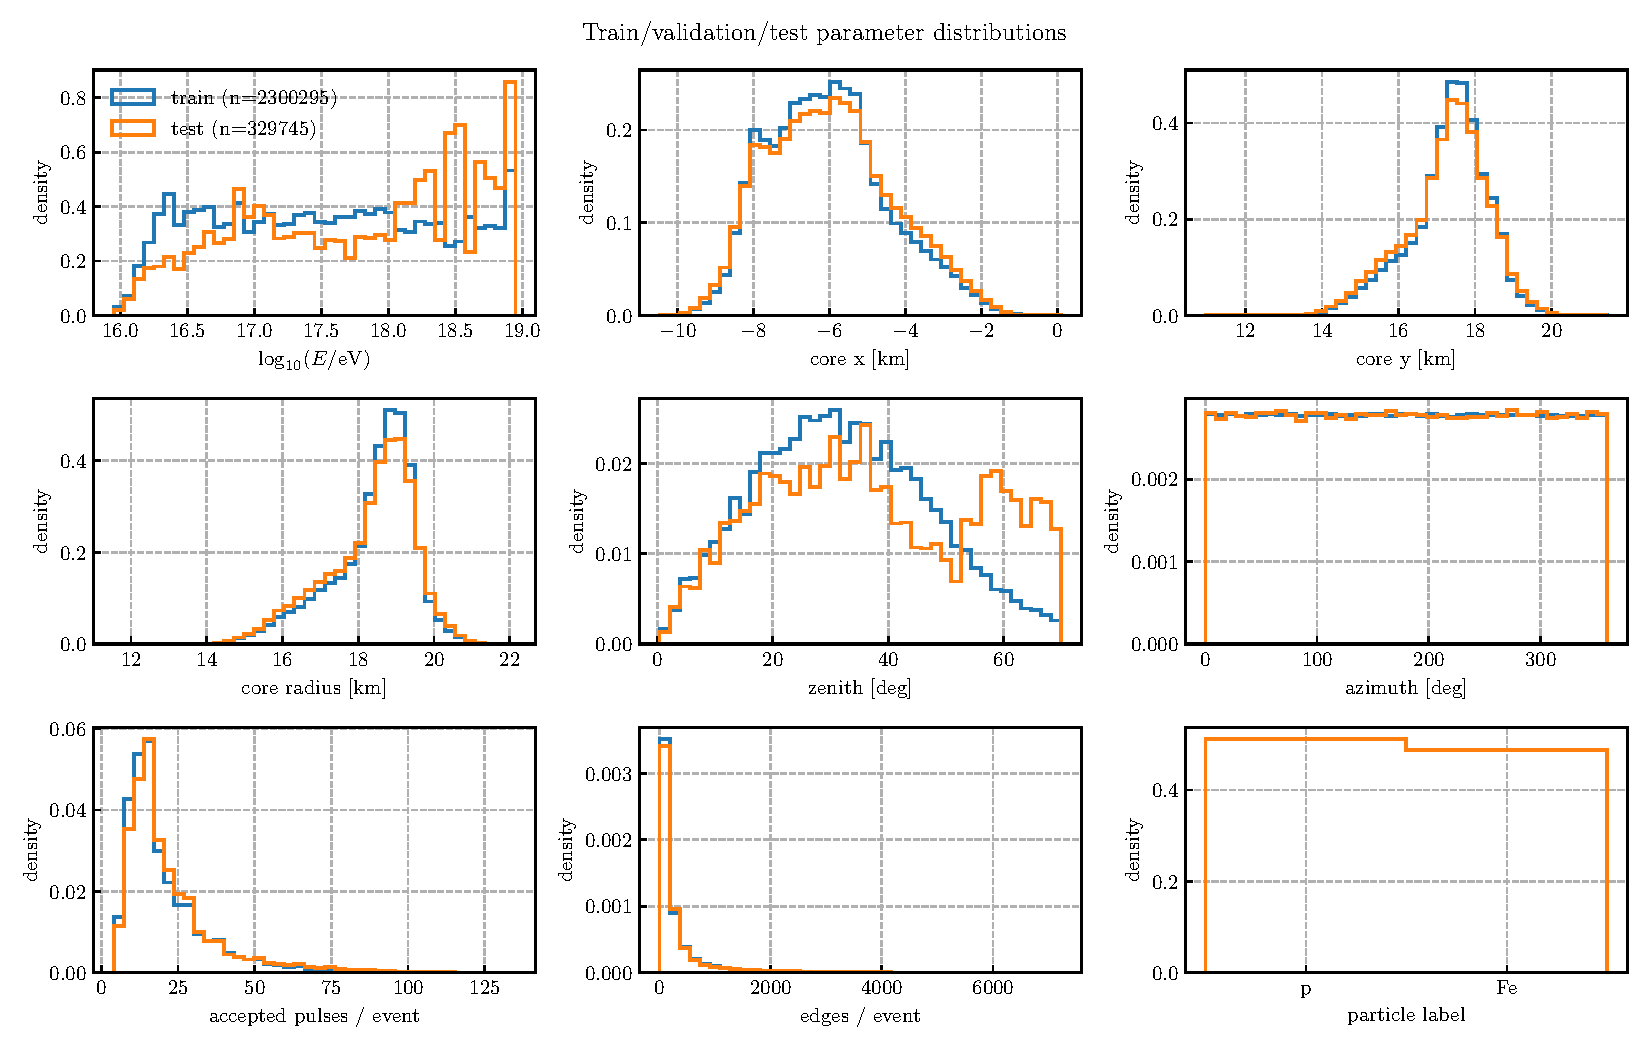
\includegraphics[width=0.95\linewidth]{fig/split_distributions/split_parameter_distributions.pdf}
  \caption{Train/validation/test distributions for the current \code{flat50000\_wfmask\_target6\_20260603\_102418} HDF5 export. Source-path separation is preserved, so the realized event fractions do not exactly match the nominal target fractions.}
  \label{fig:en-split-distributions}
\end{figure}

\clearpage
\section{Targets and Standardization}

The reconstruction target is
\[
\mathbf{y}_{\mathrm{reco}}=
(\log_{10}E,\ x_c,y_c,\ n_x,n_y,n_z)\in\R^6 .
\]
Energy is in eV and the core position is the ground-plane position in km.
The arrival direction has two physical degrees of freedom, but it is represented as a three-component unit vector to avoid angular periodicity and range constraints.
For mass classification, CORSIKA particle type 14 is mapped to proton label 0, and particle type 5626 is mapped to iron label 1.

Node, edge, and reconstruction-target scalers are fitted on the training split only.
No pulse scaler is created in the current schema because there are no additional pulse-scalar inputs.
The network predicts standardized reconstruction coordinates, but the physics loss converts predictions and targets back to physical units before computing energy, core, and angular residuals.

\section{Model Architecture}

The standard model class is \code{PhysicsTaleSdGNN}.
The current baseline uses hidden dimension $H=192$, five gated graph layers, four attentive readout heads, and a \code{cnn-gru} waveform encoder with waveform embedding dimension $D_w=64$.

\begin{figure}[p]
  \centering
  \resizebox{\linewidth}{!}{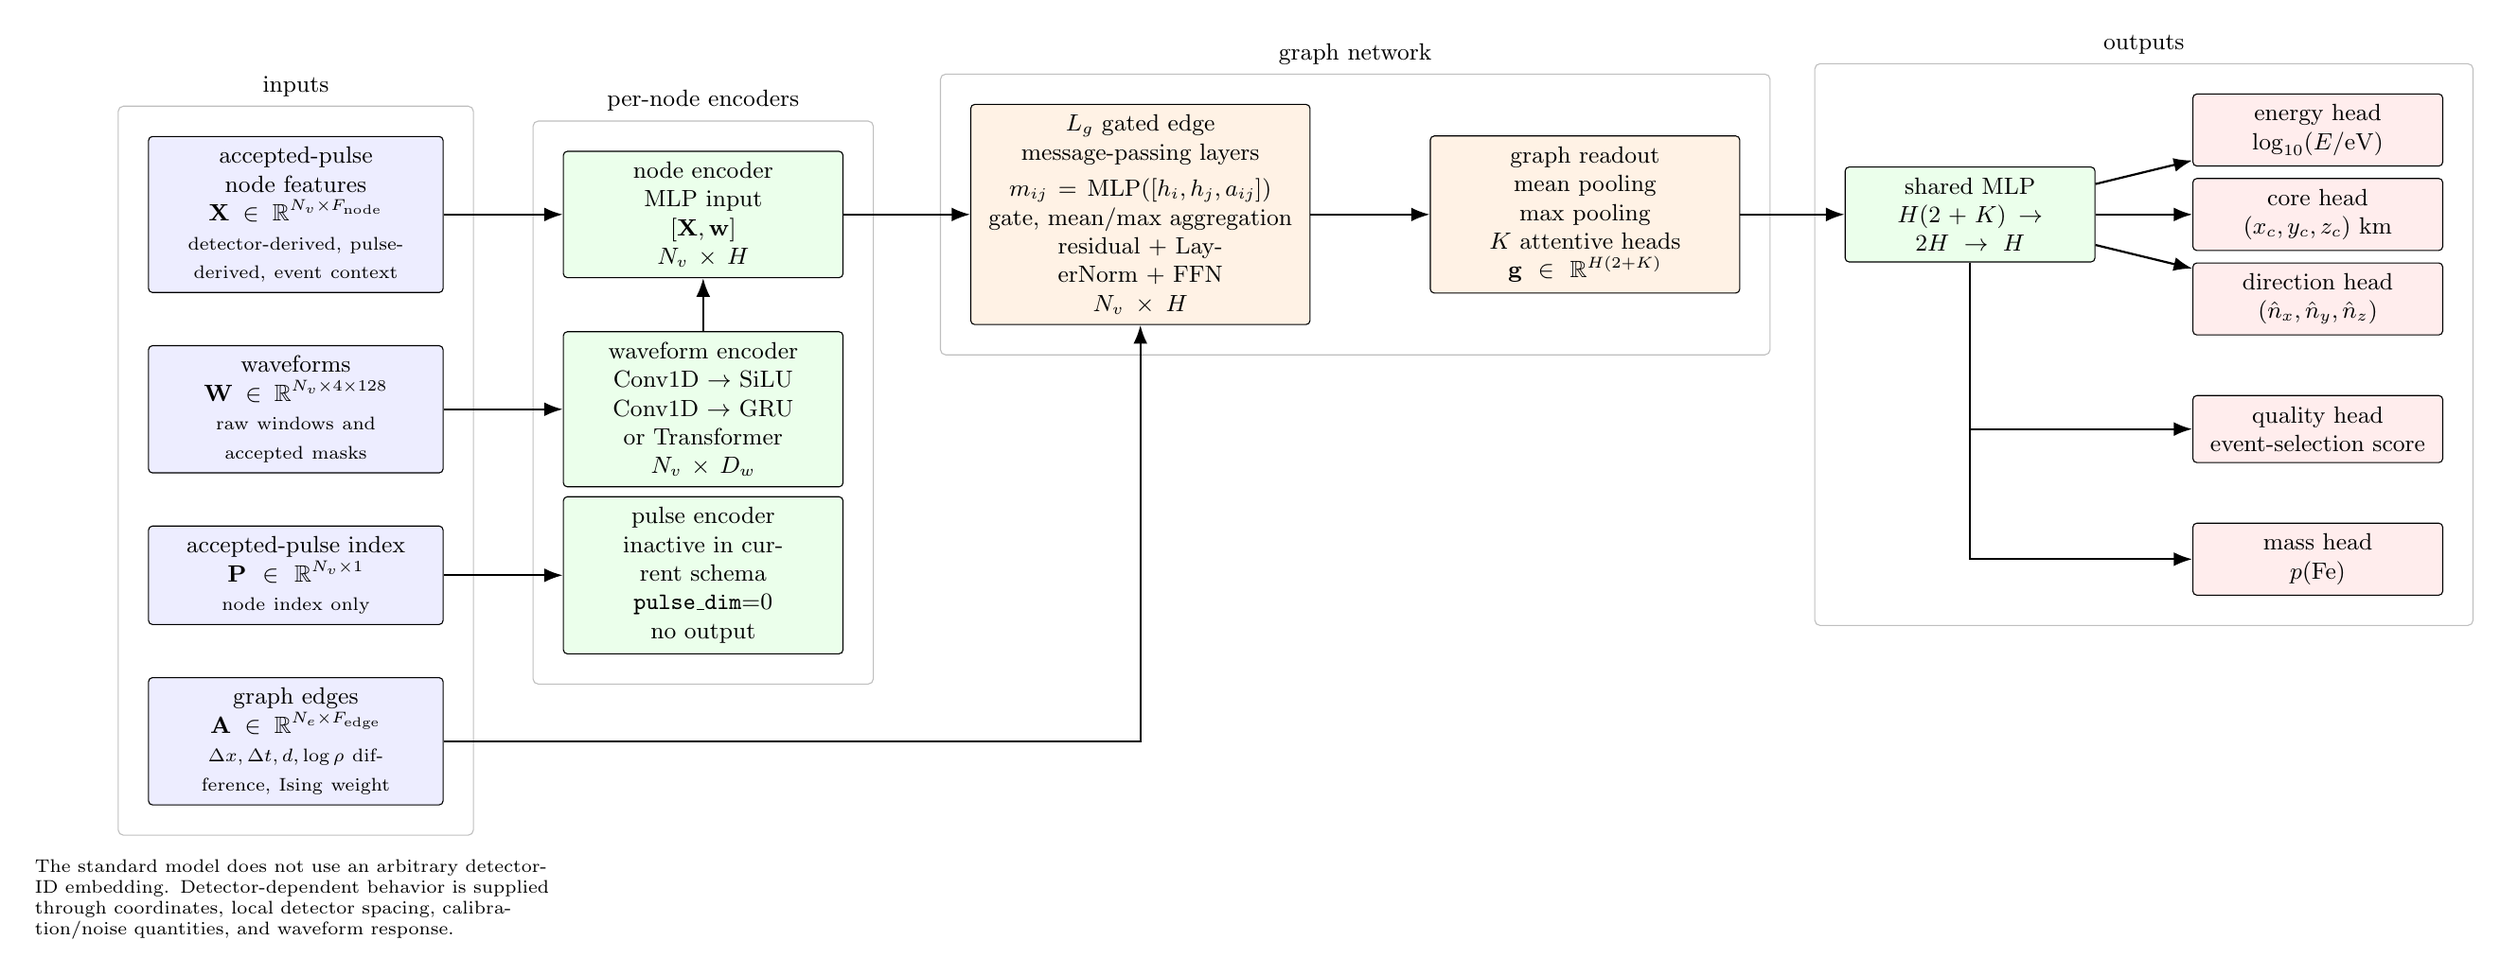
\begin{tikzpicture}[
  font=\small,
  box/.style={draw, rounded corners=1.5pt, align=center, minimum height=9mm, inner xsep=5pt, inner ysep=4pt},
  input/.style={box, fill=blue!7},
  enc/.style={box, fill=green!8},
  gnn/.style={box, fill=orange!10},
  output/.style={box, fill=red!7},
  note/.style={align=left, font=\scriptsize},
  arrow/.style={-{Latex[length=2.5mm]}, thick}
]

\node[input, text width=36mm] (x) {
  accepted-pulse node features\\
  $\mathbf{X}\in\mathbb{R}^{N_v\times F_{\mathrm{node}}}$\\
  \scriptsize detector-derived, pulse-derived, event context
};
\node[input, text width=36mm, below=7mm of x] (w) {
  waveforms\\
  $\mathbf{W}\in\mathbb{R}^{N_v\times4\times128}$\\
  \scriptsize raw windows and accepted masks
};
\node[input, text width=36mm, below=7mm of w] (p) {
  accepted-pulse index\\
  $\mathbf{P}\in\mathbb{R}^{N_v\times1}$\\
  \scriptsize node index only
};
\node[input, text width=36mm, below=7mm of p] (e) {
  graph edges\\
  $\mathbf{A}\in\mathbb{R}^{N_e\times F_{\mathrm{edge}}}$\\
  \scriptsize $\Delta x,\Delta t,d,\log\rho$ difference, Ising weight
};

\node[enc, text width=34mm, right=16mm of w] (wenc) {
  waveform encoder\\
  Conv1D $\rightarrow$ SiLU\\
  Conv1D $\rightarrow$ GRU\\
  or Transformer\\
  $N_v\times D_w$
};
\node[enc, text width=34mm, right=16mm of p] (penc) {
  pulse encoder\\
  inactive in current schema\\
  \code{pulse\_dim}=0\\
  no output
};
\node[enc, text width=34mm, right=16mm of x] (xenc) {
  node encoder\\
  MLP input\\
  $[\mathbf{X},\mathbf{w}]$\\
  $N_v\times H$
};

\node[gnn, text width=42mm, right=17mm of xenc] (mp) {
  $L_g$ gated edge\\
  message-passing layers\\
  \vspace{1mm}
  $m_{ij}=\mathrm{MLP}([h_i,h_j,a_{ij}])$\\
  gate, mean/max aggregation\\
  residual + LayerNorm + FFN\\
  $N_v\times H$
};

\node[gnn, text width=38mm, right=16mm of mp] (pool) {
  graph readout\\
  mean pooling\\
  max pooling\\
  $K$ attentive heads\\
  $\mathbf{g}\in\mathbb{R}^{H(2+K)}$
};

\node[enc, text width=30mm, right=14mm of pool] (shared) {
  shared MLP\\
  $H(2+K)\rightarrow2H\rightarrow H$
};

\node[output, text width=30mm, above right=0mm and 13mm of shared] (energy) {
  energy head\\
  $\log_{10}(E/\mathrm{eV})$
};
\node[output, text width=30mm, right=13mm of shared] (core) {
  core head\\
  $(x_c,y_c,z_c)$ km
};
\node[output, text width=30mm, below right=0mm and 13mm of shared] (dir) {
  direction head\\
  $(\hat n_x,\hat n_y,\hat n_z)$
};
\node[output, text width=30mm, below=8mm of dir] (quality) {
  quality head\\
  event-selection score
};
\node[output, text width=30mm, below=8mm of quality] (mass) {
  mass head\\
  $p(\mathrm{Fe})$
};

\draw[arrow] (w) -- (wenc);
\draw[arrow] (p) -- (penc);
\draw[arrow] (x) -- (xenc);
\draw[arrow] (wenc.north) -- (xenc.south);
\draw[arrow] (xenc) -- (mp);
\draw[arrow] (e) -| (mp);
\draw[arrow] (mp) -- (pool);
\draw[arrow] (pool) -- (shared);
\draw[arrow] (shared) -- (energy);
\draw[arrow] (shared) -- (core);
\draw[arrow] (shared) -- (dir);
\draw[arrow] (shared) |- (quality);
\draw[arrow] (shared) |- (mass);

\node[note, below=6mm of e, text width=70mm] (idnote) {
  The standard model does not use an arbitrary detector-ID embedding. Detector-dependent behavior is supplied through coordinates, local detector spacing, calibration/noise quantities, and waveform response.
};

\begin{scope}[on background layer]
  \node[draw=gray!50, rounded corners=2pt, fit=(x)(w)(p)(e), inner sep=4mm, label={[font=\small]above:inputs}] {};
  \node[draw=gray!50, rounded corners=2pt, fit=(wenc)(penc)(xenc), inner sep=4mm, label={[font=\small]above:per-node encoders}] {};
  \node[draw=gray!50, rounded corners=2pt, fit=(mp)(pool), inner sep=4mm, label={[font=\small]above:graph network}] {};
  \node[draw=gray!50, rounded corners=2pt, fit=(shared)(energy)(core)(dir)(quality)(mass), inner sep=4mm, label={[font=\small]above:outputs}] {};
\end{scope}

\end{tikzpicture}
}
  \caption{Common model flow. Detector layout is not treated as a regular image; detector information enters through physical scalar features, waveforms, and graph edges.}
  \label{fig:en-model-architecture}
\end{figure}

\begin{figure}[p]
  \centering
  \resizebox{0.92\linewidth}{!}{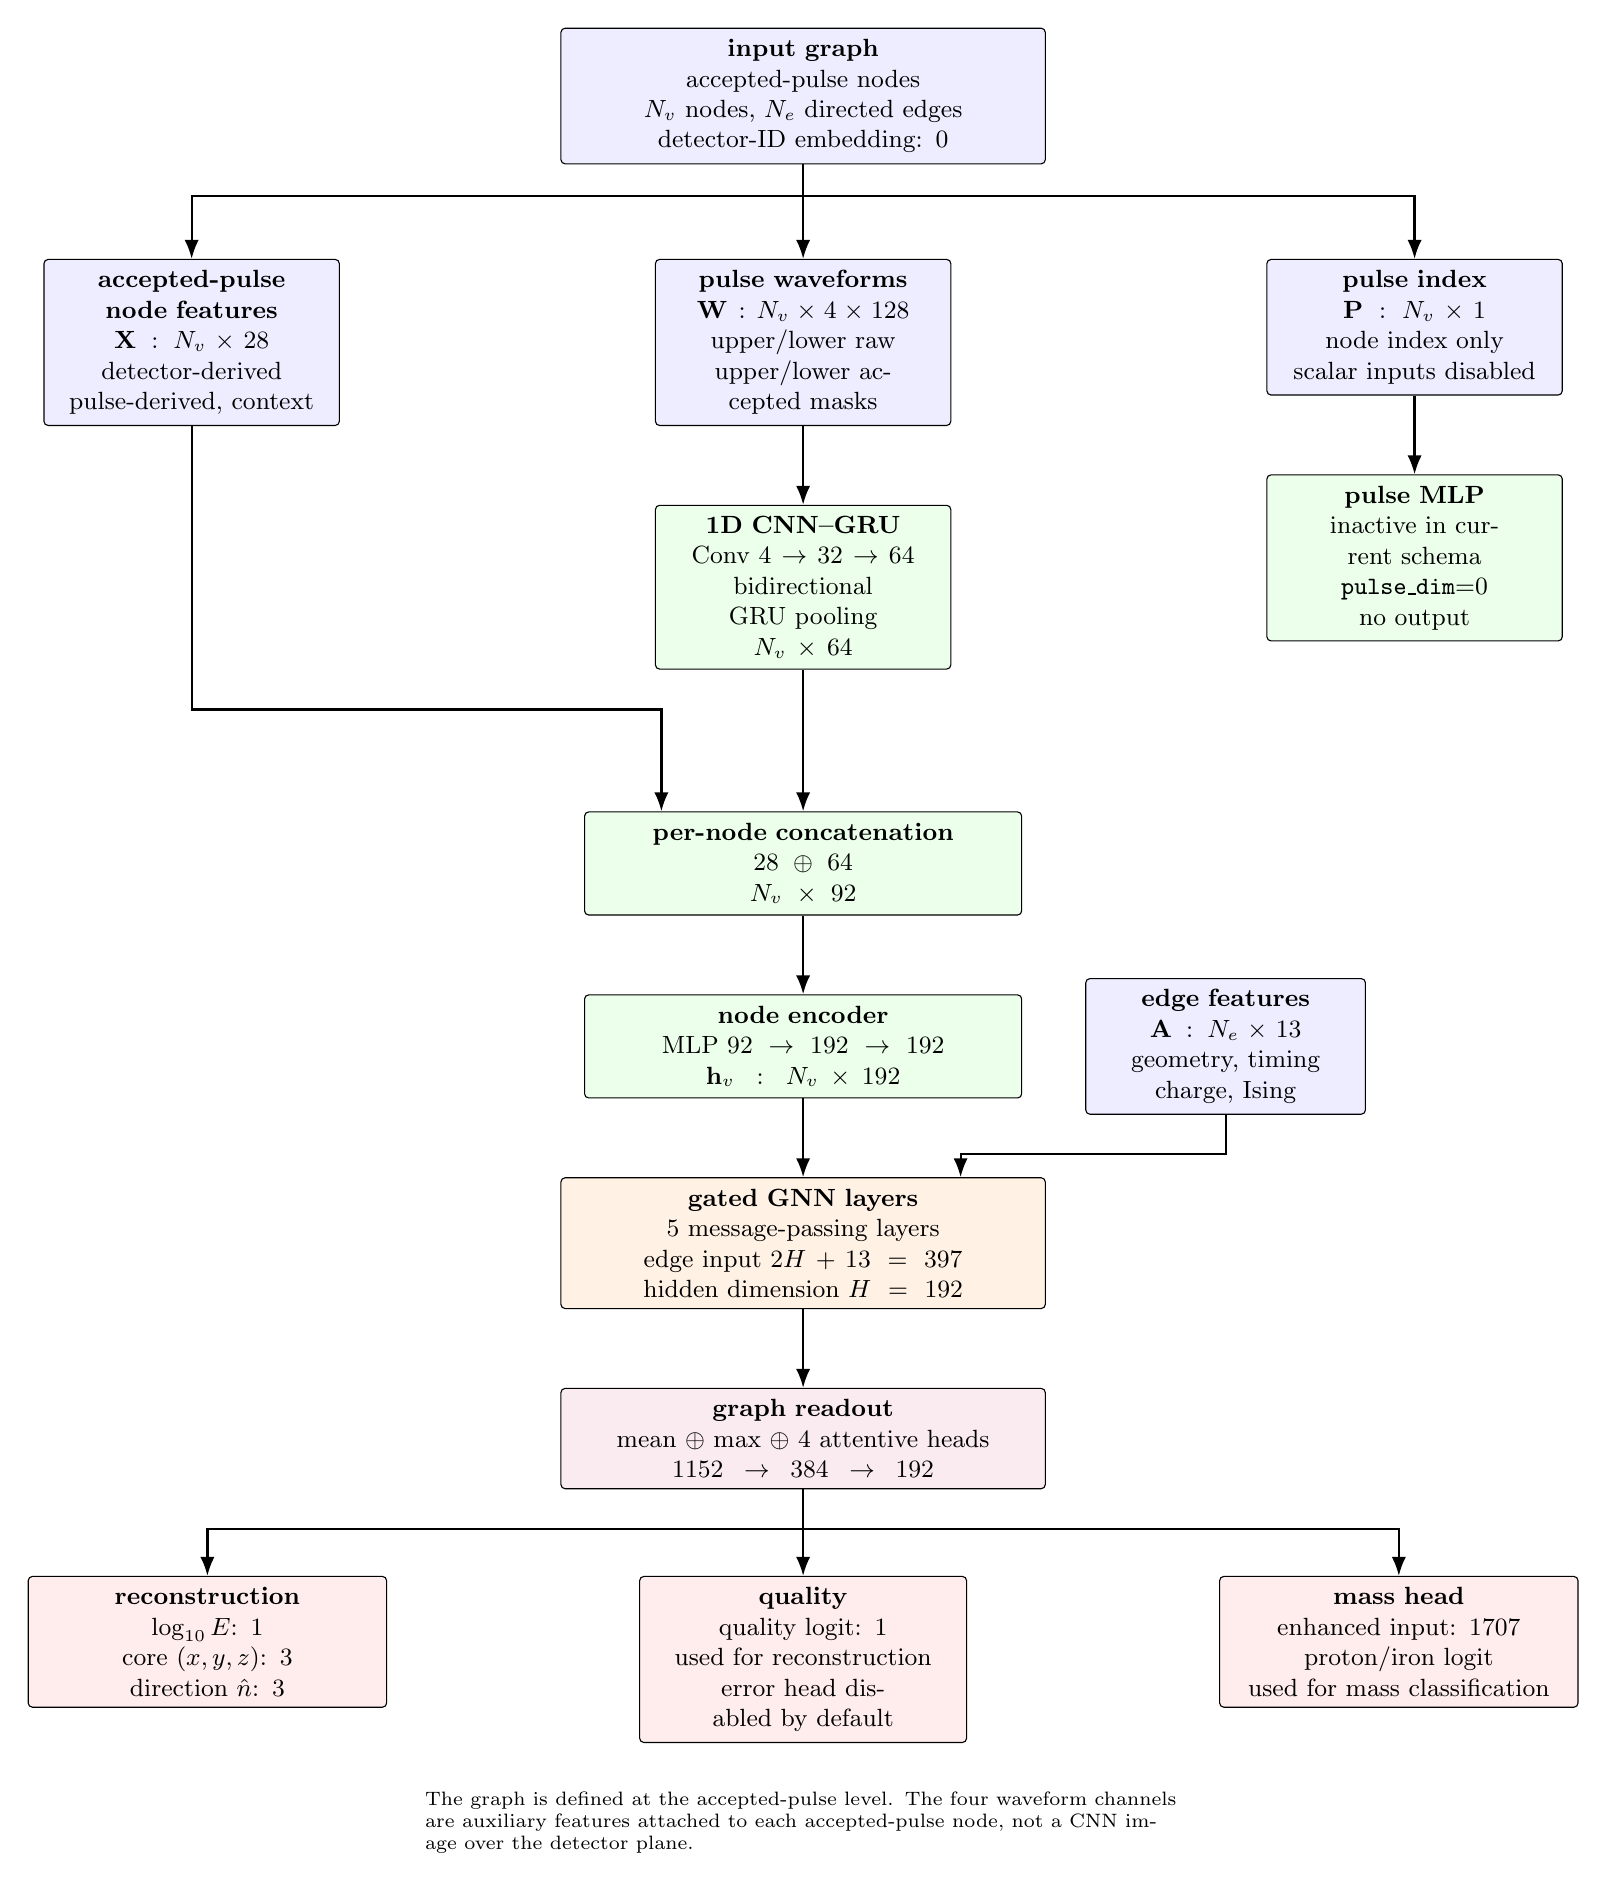
\begin{tikzpicture}[
  font=\small,
  box/.style={draw, rounded corners=1.5pt, align=center, inner xsep=5pt, inner ysep=4pt},
  input/.style={box, fill=blue!7},
  enc/.style={box, fill=green!8},
  gnn/.style={box, fill=orange!10},
  readout/.style={box, fill=purple!8},
  output/.style={box, fill=red!7},
  note/.style={align=left, font=\scriptsize},
  arrow/.style={-{Latex[length=2.4mm]}, thick}
]

\node[input, text width=58mm] (graph) at (0,0) {
  \textbf{input graph}\\
  accepted-pulse nodes\\
  $N_v$ nodes, $N_e$ directed edges\\
  detector-ID embedding: $0$
};

\node[input, text width=34mm, below left=12mm and 28mm of graph] (x) {
  \textbf{accepted-pulse}\\
  \textbf{node features}\\
  $\mathbf{X}:N_v\times28$\\
  detector-derived\\
  pulse-derived, context
};
\node[input, text width=34mm, below=12mm of graph] (w) {
  \textbf{pulse waveforms}\\
  $\mathbf{W}:N_v\times4\times128$\\
  upper/lower raw\\
  upper/lower accepted masks
};
\node[input, text width=34mm, below right=12mm and 28mm of graph] (p) {
  \textbf{pulse index}\\
  $\mathbf{P}:N_v\times1$\\
  node index only\\
  scalar inputs disabled
};

\node[enc, text width=34mm, below=10mm of w] (wenc) {
  \textbf{1D CNN--GRU}\\
  Conv $4\to32\to64$\\
  bidirectional GRU pooling\\
  $N_v\times64$
};
\node[enc, text width=34mm, below=10mm of p] (penc) {
  \textbf{pulse MLP}\\
  inactive in current schema\\
  \code{pulse\_dim}=0\\
  no output
};

\node[enc, text width=52mm, below=18mm of wenc] (concat) {
  \textbf{per-node concatenation}\\
  $28\oplus64$\\
  $N_v\times92$
};
\node[enc, text width=52mm, below=10mm of concat] (nenc) {
  \textbf{node encoder}\\
  MLP $92\to192\to192$\\
  $\mathbf{h}_v:N_v\times192$
};

\node[input, text width=32mm, right=8mm of nenc] (edge) {
  \textbf{edge features}\\
  $\mathbf{A}:N_e\times13$\\
  geometry, timing\\
  charge, Ising
};

\node[gnn, text width=58mm, below=10mm of nenc] (mp) {
  \textbf{gated GNN layers}\\
  $5$ message-passing layers\\
  edge input $2H+13=397$\\
  hidden dimension $H=192$
};

\node[readout, text width=58mm, below=10mm of mp] (readout) {
  \textbf{graph readout}\\
  mean $\oplus$ max $\oplus$ $4$ attentive heads\\
  $1152\to384\to192$
};

\node[output, text width=42mm, below left=11mm and 22mm of readout] (reco) {
  \textbf{reconstruction}\\
  $\log_{10}E$: $1$\\
  core $(x,y,z)$: $3$\\
  direction $\hat{n}$: $3$
};
\node[output, text width=38mm, below=11mm of readout] (quality) {
  \textbf{quality}\\
  quality logit: $1$\\
  used for reconstruction\\
  error head disabled by default
};
\node[output, text width=42mm, below right=11mm and 22mm of readout] (mass) {
  \textbf{mass head}\\
  enhanced input: $1707$\\
  proton/iron logit\\
  used for mass classification
};

\draw[arrow] (graph.south) -- ++(0,-4mm) -| (x.north);
\draw[arrow] (graph.south) -- (w.north);
\draw[arrow] (graph.south) -- ++(0,-4mm) -| (p.north);
\draw[arrow] (w) -- (wenc);
\draw[arrow] (p) -- (penc);
\draw[arrow] (x.south) -- ++(0,-36mm) -| ([xshift=-18mm]concat.north);
\draw[arrow] (wenc.south) -- (concat.north);
\draw[arrow] (concat) -- (nenc);
\draw[arrow] (nenc) -- (mp);
\draw[arrow] (edge.south) -- ++(0,-5mm) -| ([xshift=20mm]mp.north);
\draw[arrow] (mp) -- (readout);
\draw[arrow] (readout.south) -- ++(0,-5mm) -| (reco.north);
\draw[arrow] (readout.south) -- (quality.north);
\draw[arrow] (readout.south) -- ++(0,-5mm) -| (mass.north);

\node[note, below=5mm of quality.south, text width=96mm, anchor=north] {
  The graph is defined at the accepted-pulse level. The four waveform channels are auxiliary features attached to each accepted-pulse node, not a CNN image over the detector plane.
};

\end{tikzpicture}
}
  \caption{Concrete baseline used by the current training scripts. Reconstruction and mass-classification modes share the encoders and GNN, and switch the active heads and loss terms.}
  \label{fig:en-concrete-training-model}
\end{figure}

\subsection{Node Encoders}

In the current schema, \code{pulse\_features} contains only \code{node\_index}, so \code{pulse\_dim=0}; the pulse encoder and pulse pooling branch are inactive.

The waveform encoder applies two one-dimensional convolution blocks to the four waveform channels, followed by a bidirectional GRU in the standard mode.
The final GRU state, the mean of the convolutional sequence, and the max of the convolutional sequence are concatenated and projected to a 64-dimensional waveform embedding.

The node encoder concatenates the 28 accepted-pulse node scalar features and the 64-dimensional waveform embedding:
\[
  28\oplus64=92.
\]
This vector is mapped to the hidden node state with a two-layer MLP,
\[
  \R^{92}\rightarrow\R^{192}\rightarrow\R^{192}.
\]
SiLU activations and layer normalization are used in the node encoder.

\subsection{Message Passing and Readout}

Before the graph layers, a time-difference encoder processes the edge timing features
$(\Delta t,|\Delta t|,\Delta t/d)$
and adds their destination-node average to the node state.
This gives the shower-front timing information a direct path into the node representation.

For each directed edge $i\rightarrow j$, the gated message layer uses
\[
  [h_i,h_j,a_{ij}]\in\R^{2H+13}
\]
as input.
The message is
\[
  m_{ij}=
  \mathrm{MLP}_m([h_i,h_j,a_{ij}])\,
  \sigma(\mathrm{MLP}_g([h_i,h_j,a_{ij}])).
\]
Incoming messages are summarized by both mean and max aggregation.
The node update uses a residual connection, layer normalization, and a feed-forward block.

After five graph layers, the graph readout concatenates global mean pooling, global max pooling, and four attentive readout heads.
The event vector therefore has dimension
\[
  H(2+4)=1152.
\]
For reconstruction and quality prediction, this vector is passed through a shared MLP
\[
  \R^{1152}\rightarrow\R^{384}\rightarrow\R^{192}.
\]

\section{Outputs}

The reconstruction heads predict
\[
(\widehat{\log_{10}E},\hat{x}_c,\hat{y}_c,\hat{n}_x,\hat{n}_y,\hat{n}_z).
\]
The energy head is linear.
The core head predicts the horizontal ground-plane core coordinates.
The direction head predicts a three-component direction vector.
When angular residuals are computed, the predicted and true direction vectors are normalized internally.

The quality head outputs one logit $q_{\mathrm{logit}}$.
The event quality score is $\sigma(q_{\mathrm{logit}})$ and is used as an event-selection score for reconstruction analyses.

The enhanced mass-classification head outputs one logit $z_{\mathrm{mass}}$.
The iron probability is
\[
  p(\mathrm{Fe})=\sigma(z_{\mathrm{mass}}).
\]
The enhanced head uses the final graph readout, the initial node-encoder readout, graph-size context, and direct waveform summaries.
With the current dimensions, its input dimension is 1707.

An optional error-prediction head exists, but it is not part of the current baseline.

\section{Loss Functions}

For a residual $r$, the SmoothL1 loss is
\[
  \mathrm{SmoothL1}_{\beta}(r)=
  \begin{cases}
    r^2/(2\beta), & |r|<\beta,\\
    |r|-\beta/2, & |r|\ge\beta.
  \end{cases}
\]
For a logit $z$ and target $y\in[0,1]$,
\[
  \mathrm{BCEWithLogits}(z,y)
  =
  -y\log\sigma(z)-(1-y)\log(1-\sigma(z)).
\]
The same BCEWithLogits expression is used both for binary mass labels and for continuous quality soft targets.

\subsection{Physics Reconstruction Loss}

The physics reconstruction loss is
\[
  L_{\mathrm{phys}} =
  w_E L_E + w_c L_c + w_\theta L_\theta,
\]
with the current weights
\[
  w_E=1.2,\qquad w_c=1.0,\qquad w_\theta=1.4.
\]
The energy term is
\[
  L_E=
  \mathrm{SmoothL1}(\widehat{\log_{10}E}-\log_{10}E;\beta=0.05).
\]
The core term uses the horizontal core residual:
\[
  L_c=
  \left\langle
  \frac{(\hat{x}_c-x_c)^2+(\hat{y}_c-y_c)^2}
       {(0.05\,\mathrm{km})^2}
  \right\rangle.
\]
The direction term uses the angular separation $\alpha$ between the predicted and true directions:
\[
  L_\theta=
  \mathrm{SmoothL1}\left(\frac{\alpha}{1.0^\circ};\beta=1\right).
\]

\subsection{Energy Bias Penalties}

To suppress a positive low-energy bias in
$\widehat{\log_{10}E}-\log_{10}E$, the next reconstruction training condition
adds supervised penalties on the mean log-energy residual in true-energy bins.
These terms are training losses for MC-labeled data, not post-hoc corrections for real data.
Let
\[
  \delta_i=\widehat{\log_{10}E_i}-\log_{10}E_i
\]
and let $B_k$ be bins in true $\log_{10}E$ with width 0.1. The bin-mean bias term is
\[
  L_{\mathrm{bias}}=
  \left\langle
  \left(
  \frac{1}{|B_k|}\sum_{i\in B_k}\delta_i
  \right)^2
  \right\rangle_k .
\]
To prevent proton and iron biases from cancelling each other inside the same energy bin, the training loss also includes
\[
  L_{\mathrm{p/Fe}}=
  \left\langle
  \left(
  \langle\delta\rangle_{B_k,\mathrm{proton}}
  -
  \langle\delta\rangle_{B_k,\mathrm{iron}}
  \right)^2
  \right\rangle_k .
\]
The default submitters for reconstruction-containing runs use
\[
  \lambda_{\mathrm{bias}}=1.0,\qquad
  \lambda_{\mathrm{p/Fe}}=1.0.
\]

\subsection{Quality Loss}

The quality target is computed from the current reconstruction residual and detached from the computation graph:
\[
  q_{\mathrm{target}}=
  \exp\left[-\frac{1}{3}\left(
  \frac{|E_{\mathrm{rec}}/E_{\mathrm{true}}-1|}{0.10}
  +\frac{\Delta r_c}{0.05\,\mathrm{km}}
  +\frac{\alpha}{1.0^\circ}
  \right)\right].
\]
The quality loss is
\[
  L_q=\mathrm{BCEWithLogits}(q_{\mathrm{logit}},q_{\mathrm{target}}),
  \qquad w_q=0.2.
\]
For reconstruction without mass classification, the total loss is
\[
  L_{\mathrm{reco}}
  =
  L_{\mathrm{phys}}
  +\lambda_{\mathrm{bias}}L_{\mathrm{bias}}
  +\lambda_{\mathrm{p/Fe}}L_{\mathrm{p/Fe}}
  +0.2\,L_q.
\]

\subsection{Mass Classification Loss}

The default mass-classification loss is BCEWithLogits with proton label 0 and iron label 1:
\[
  L_{\mathrm{BCE}}=
  -y\log\sigma(z_{\mathrm{mass}})
  -(1-y)\log(1-\sigma(z_{\mathrm{mass}})).
\]
No additional positive-class weight is used in the current baseline.

The implementation also supports focal loss:
\[
  L_{\mathrm{focal}}=
  \left\langle
  (1-p_{t,i})^\gamma
  \mathrm{BCEWithLogits}(z_i,y_i)
  \right\rangle_i,
\]
where $p_{t,i}=p_i$ for iron events and $p_{t,i}=1-p_i$ for proton events.

When both proton and iron events appear in a batch, a ranking term can be added:
\[
  L_{\mathrm{rank}}=
  \left\langle
  \mathrm{softplus}\left(m-(z^+-z^-)\right)
  \right\rangle,
\]
where $z^+$ is an iron logit, $z^-$ is a proton logit, and the current margin is $m=1.0$.
The current mass baseline uses
\[
  L_{\mathrm{mass}}=L_{\mathrm{BCE}}+0.5\,L_{\mathrm{rank}}.
\]

\subsection{Joint Reco+Mass Objective}

The joint baseline combines reconstruction, quality, and mass terms:
\[
  L_{\mathrm{total}}
  =
  L_{\mathrm{phys}}
  +\lambda_{\mathrm{bias}}L_{\mathrm{bias}}
  +\lambda_{\mathrm{p/Fe}}L_{\mathrm{p/Fe}}
  +0.2\,L_q
  +\lambda_{\mathrm{mass}} L_{\mathrm{mass}}.
\]
The current candidate setting is
\[
  \lambda_{\mathrm{mass}}=0.15,\qquad
  L_{\mathrm{mass}}=L_{\mathrm{BCE}}+0.5\,L_{\mathrm{rank}}.
\]
This weight was chosen from the observed loss scale of an earlier joint run, where the previous mass weight of 0.05 made the mass term much smaller than the quality term.

\subsection{Optional Error/NLL Mode}

The code can predict event-wise expected errors and combine them with a Gaussian negative log-likelihood.
This mode is currently not the baseline.
The present baseline keeps error prediction disabled and uses the detached quality score as the event-selection output.

\section{Evaluation Outputs}

After training, the best validation checkpoint is loaded before final validation and test evaluation.
The main reconstruction metrics are energy residuals in $\log_{10}E$, angular resolution, and core-position resolution.
Quality-cut curves are used to show how resolution changes as low-quality events are removed.
For mass classification, the main metrics are accuracy, balanced accuracy, ROC AUC, score distributions, and confusion matrices.

\end{document}
